\documentclass[12pt,a4paper]{report}
\usepackage[utf8]{inputenc}
\usepackage[greek,english]{babel}
\usepackage{alphabeta}
\usepackage{graphicx}
\usepackage{amsmath}
\usepackage{amssymb}
\usepackage{geometry}
\usepackage{float}
\usepackage{multicol}
\usepackage[ruled]{algorithm2e}
\usepackage[style=numeric, sorting=none, backend=biber]{biblatex}
\addbibresource{bibliography.bib}
\geometry{a4paper, margin=1in}
\renewcommand{\arraystretch}{1.2}

\usepackage{xcolor} % Required for colors
\usepackage{todonotes}
% --- ΡΥΘΜΙΣΕΙΣ HYPERLINKS ---
\usepackage[hidelinks, unicode]{hyperref} % unicode για σωστά ελληνικά στα bookmarks

\begin{document}
	
	% --- ENGLISH TITLE PAGE ---
	\begin{titlepage}
		\centering
		\Large \textbf{TECHNICAL UNIVERSITY OF CRETE} \\
		\large SCHOOL OF ELECTRICAL AND COMPUTER ENGINEERING \\
		\vfill
		\huge \textbf{COALITION FORMATION IN PREDATORS-PREY ENVIRONMENTS} \\
		\vfill
		\large DIPLOMA THESIS \\
		\vfill
		\Large \textbf{Georgios Angelopoulos} \\
		\vfill
		\large \textbf{COMMITTEE:} \\
		GEORGIOS CHALKIADAKIS, Associate Professor (ECE) \\
		AIKATERINI MANIA, Associate Professor (ECE) \\
		MICHAIL G. LAGOUDAKIS, Associate Professor (ECE)
		\vfill
		\large Chania, February 2026
	\end{titlepage}
	
	% --- GREEK TITLE PAGE ---
	\begin{titlepage}
		\selectlanguage{greek}
		\centering
		\Large \textbf{ΠΟΛΥΤΕΧΝΕΙΟ ΚΡΗΤΗΣ} \\
		\large ΣΧΟΛΗ ΗΛΕΚΤΡΟΛΟΓΩΝ ΜΗΧΑΝΙΚΩΝ ΚΑΙ ΜΗΧΑΝΙΚΩΝ ΥΠΟΛΟΓΙΣΤΩΝ \\
		\vfill
		\huge \textbf{ΔΗΜΙΟΥΡΓΙΑ ΣΥΝΑΣΠΙΣΜΩΝ ΣΕ ΠΕΡΙΒΑΛΛΟΝΤΑ ΘΗΡΕΥΣΗΣ ΑΠΟ ΟΜΑΔΕΣ} \\
		\vfill
		\large ΔΙΠΛΩΜΑΤΙΚΗ ΕΡΓΑΣΙΑ \\
		\vfill
		\Large \textbf{Γεώργιος Αγγελόπουλος} \\
		\vfill
		\large \textbf{ΕΠΙΤΡΟΠΗ:} \\
		ΓΕΩΡΓΙΟΣ ΧΑΛΚΙΑΔΑΚΗΣ, Αναπληρωτής Καθηγητής (ΗΜMY) \\
		ΑΙΚΑΤΕΡΙΝΗ ΜΑΝΙΑ, Αναπληρώτρια Καθηγήτρια (ΗΜΜΥ) \\
		ΜΙΧΑΗΛ Γ. ΛΑΓΟΥΔΑΚΗΣ, Αναπληρωτής Καθηγητής (ΗΜΜΥ)
		\vfill
		\large Χανιά, Φεβρουάριος 2026
		\selectlanguage{english}
	\end{titlepage}
	
	% --- ΠΡΟΚΑΤΑΡΚΤΙΚΕΣ ΣΕΛΙΔΕΣ (Λατινική αρίθμηση) ---
	\pagenumbering{roman}
	\cleardoublepage
	
	% Abstract (English)
	\chapter*{Abstract}
	\addcontentsline{toc}{chapter}{Abstract}
	
	Cooperative Game theory and multi-agent systems have long focused on how autonomous individuals can form stable coalitions to achieve shared goals. However, an unresolved question arises as to what principles determine the effectiveness of reward sharing mechanisms in agent social welfare. This thesis investigates utility distribution tactics in ecology-inspired multi-agent systems. Specifically, we examine how different distribution strategies maximize social welfare while preserving agent rationality in realistic, dynamic scenarios such as a predators-prey hunting simulation. \\   
	
	This thesis consists of two distinct parts. In the first part, we develop a novel simulated environment that focuses on mimicking a natural, realistic ecology where rational "predator" agents interact and hunt passive "prey" agents on a spatial hexagonal grid area. We then systematically compare the overall performance of predators across an extensive array of simulated episodes, altering the underlying reward distribution tactic in each scenario to observe its impact on agent cooperation and overall social welfare. This comparative analysis provides key academic insights into which distributive principles most effectively maximize cooperation and prevent coordination deadlocks in heterogeneous agent populations. \\
	
	In the second part, we have designed and implemented a serious game application that uses our simulated environment. Through the player's actions, it acts as a visual and entertaining introduction to foundational concepts of multi-agent environments, utility-based rationality and the logic behind coalition bargaining. \\
	
	% Περίληψη (Ελληνικά)
	\selectlanguage{greek}
	\chapter*{Περίληψη}
	\addcontentsline{toc}{chapter}{Περίληψη}
	Η Συνεργατική Θεωρία Παιγνίων και τα συστήματα πολλαπλών πρακτόρων εστιάζουν εδώ και καιρό στο πώς αυτόνομες οντότητες μπορούν να σχηματίσουν σταθερούς συνασπισμούς για την επίτευξη κοινών στόχων. Ωστόσο, προκύπτει ένα άλυτο ερώτημα σχετικά με το ποιες αρχές καθορίζουν την αποτελεσματικότητα των μηχανισμών διαμοιρασμού ανταμοιβών στην κοινωνική ευημερία των πρακτόρων. Η παρούσα διπλωματική εργασία διερευνά τις τακτικές κατανομής ανταμοιβών σε συστήματα πολλαπλών πρακτόρων εμπνευσμένα από την οικολογία. Συγκεκριμένα, εξετάζουμε πώς διαφορετικές στρατηγικές κατανομής μεγιστοποιούν την κοινωνική ευημερία, διατηρώντας παράλληλα την ορθολογικότητα των πρακτόρων σε ρεαλιστικά, δυναμικά σενάρια, όπως μια προσομοίωση κυνηγιού θηρευτών-θηραμάτων. \\
	
	Η παρούσα εργασία αποτελείται από δύο διακριτά μέρη. Στο πρώτο μέρος, αναπτύσουμε ένα νέο περιβάλλον προσομοίωσης που επικεντρώνεται στη μίμηση μιας φυσικής, ρεαλιστικής οικολογίας, όπου ορθολογικοί πράκτορες-«θηρευτές» αλληλεπιδρούν και κυνηγούν παθητικούς πράκτορες-«θηράματα» σε μια περιοχή χωρικού εξαγωνικού πλέγματος. Στη συνέχεια, συγκρίνουμε συστηματικά τη συνολική απόδοση των θηρευτών σε ένα εκτενές σύνολο προσομοιωμένων επεισοδίων, μεταβάλλοντας την καθολική τακτική κατανομής ανταμοιβής σε κάθε σενάριο, προκειμένου να παρατηρήσουμε τον αντίκτυπό της στη συνεργασία των πρακτόρων και τη συνολική κοινωνική ευημερία. Αυτή η συγκριτική ανάλυση προσφέρει βασικές ακαδημαϊκές γνώσεις σχετικά με το ποιες διανεμητικές αρχές μεγιστοποιούν αποτελεσματικότερα τη συνεργασία και αποτρέπουν τα αδιέξοδα συντονισμού σε ετερογενείς πληθυσμούς πρακτόρων. \\
	
	Στο δεύτερο μέρος, σχεδιάσαμε και υλοποιήσαμε μια εφαρμογή παιχνιδιού σοβαρού σκοπού, η οποία χρησιμοποιεί το περιβάλλον προσομοίωσής μας. Μέσα από τις ενέργειες του παίκτη, η εφαρμογή λειτουργεί ως μια οπτική και ψυχαγωγική εισαγωγή σε θεμελιώδεις έννοιες των περιβαλλόντων πολλαπλών πρακτόρων, της ορθολογικότητας που βασίζεται στη χρησιμότητα και της λογικής πίσω από τη διαπραγμάτευση συνασπισμών.
	\selectlanguage{english}
	
	% Ευχαριστίες (Προαιρετικό)
	\chapter*{Acknowledgements}
	\addcontentsline{toc}{chapter}{Acknowledgements}
	
	
	% --- ΠΙΝΑΚΑΣ ΠΕΡΙΕΧΟΜΕΝΩΝ ---
	% Τα hyperlinks θα δημιουργηθούν αυτόματα εδώ
	\tableofcontents
	\newpage
	
	\listoffigures
	\listoftables
	\listofalgorithms
	\newpage
	
	% --- ΚΥΡΙΟ ΜΕΡΟΣ (Αραβική αρίθμηση) ---
	\clearpage
	\pagenumbering{arabic}
	
%-----------------------------------------------------
%--------------- Introduction Chapter ----------------
%-----------------------------------------------------
	\chapter{Introduction}
	\label{ch:intro}
	Your introduction starts here. You can use sections to organize your thoughts.
	
	\section{Contributions}
	What this thesis aims to achieve...
	
	\section{Thesis Outline}
	
	Here we give a brief overview of the content of the thesis. In Chapter 2, we present the theoretical background that is essential for understanding the various terms used and technicalities regarding artificial intelligence, multi-agent systems and coalition formation. In Chapter 3, ... In Chapter 4, we run and analyze a series of experiments   
	
%-----------------------------------------------------
%---------------- Background Chapter -----------------
%-----------------------------------------------------
	\chapter{Theoretical Background}
	\label{ch:background}
	
	In this chapter, we introduce the theoretical concepts that are necessary to understand the design decisions we made throughout this thesis. These technicalities are tied to specific principles that our simulation environment and coalition formation framework directly build upon in Chapter 3. We begin with a brief overview of multi-agent systems and the notion of a rational, utility-maximizing agent, the underlying behavior of our predator agents in our environment. We then turn to cooperative game theory, covering the structure of coalitions, the non-cooperative bargaining model of our negotiation protocol and the competing principles of distributive justice that our reward allocation tactics are based on. Finally, we introduce the notions of multi-agent reward design, resource-bounded rationality, and spatial representation in agent-based models.
	
	\section{Multi-Agent Systems and Rationality}
	
	
	
	\section{Cooperative Game Theory and Coalition Formation}
	
	\subsection{Non-Cooperative Bargaining over Coalitions}
	\subsection{Distributive Justice in Reward Allocation}
	
	\section{Multi-Agent Reward Design}
	
	\section{Resource-Bounded Rationality}
	
	\section{Spatial Representation for Agent-Based Models}
	
	\chapter{Simulation Environment}
	\label{ch:approach}
	In this chapter, we present the complete design of our simulation environment. We first introduce the topology of our agents' interactions, followed by the overview of our passive "Prey" agents. Then, we define thoroughly our rational "Predator" agents, focusing on how their expected utility computation drives their decision-making and action execution. Finally, we lay the foundation for the Predators' coalition formation logic that take place during cooperative hunts.   
	
	\section{Hexagonal Spatial Topology}
	
	To simplify and better evaluate agent behaviors within our custom environment, the spatial area is designed as a discrete, non-rendered hexagonal pattern utilizing an Axial Coordinate System \cite{Patel2016}. Each individual hex node is assigned a tuple of unique coordinates $(q, r) \in \mathbb{Z}^2$. Mathematically, for a map radius of $R$, the set of valid Hex nodes $H$ comprising the environment is defined as: \\
	
	\[H = \{ (q, r) \in \mathbb{Z}^2 \mid |q| \le R, \, |r| \le R, \, |q + r| \le R \} \] \\
	
	Currently, our simulation uses a map radius of $R = 5$. This algebraic definition yields a finite graph structure without requiring a graphical rendering pipeline during the experimental stage of our work. While the geometric properties are covered via these coordinate tuples, the rendered Hexagonal Mesh generation needed for the serious game implementation is elaborated in detail in section 5.2. \\
	
	The main advantage of utilizing a hexagonal topology over a traditional Cartesian square grid is its uniform connectivity, since the euclidean distance between the center of any given hex node and its six immediate neighbors is perfectly isometric \cite{Patel2016}. This spatial uniformity simplifies agent movement and ensures that all moving actions incur a uniform metabolic cost, which is assigned globally at simulation start. All agent transitions are strictly discrete, occurring from their current hex node to an adjacent one. \\
	
	Furthermore, this axial coordinates system provides high computational efficiency by eliminating continuous floating-point spatial calculations and removing complex edge-cases regarding boundary overlap or continuous proximity detection. Agent interactions are instead governed entirely by node co-location. Under this principle, multiple predators and prey are permitted to simultaneously occupy the same coordinates $(q, r)$. This logic serves as the requirement for all high-level agent interactions, as predator hunting mechanisms and coalition bargaining can only execute if the participating agents occupy identical axial coordinates. \\
	
	\begin{figure}[H]
		\centering
		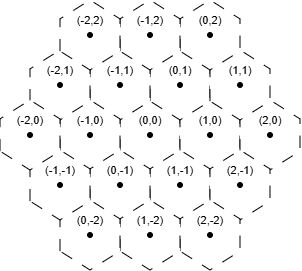
\includegraphics[width=0.5\textwidth]{HexTopology.png}
		\caption{Hexagonal Spatial Topology Example (R=2).}
		\label{fig:hex_topology}
	\end{figure}
	  
	\section{Prey Agents}

	Prey Agents passively roam the simulation. They are the hunting targets of Predator agents since successfully capturing prey yields rewards that replenish the predator's energy reserves. Thus, they are also the focus of potential predators' coalition formation and cooperative hunts. In this section, we define the basic prey types and their respected parameters and offer a brief introduction to their simple action cycle. \\
	
	\subsection{Prey Types}
	
	Each Prey $a$ is defined by a fixed type vector that compromises its characteristics in a hunt scenario. Besides that, they are identical in how they move or being interacted with. At every simulated episode setup, each prey agent is assigned a specific type at random. Depending on this type, the rest of the parameters are assigned automatically: \\
	
	\[{Prey}_a = \langle Type_a, P_{solo,a}, R_{a}, β_{α} \rangle\] \\
	
	\begin{itemize}
		\item The "Hare" represents the smallest and safest hunting option with high success chance and low reward, with a baseline synergy factor.
		
		\item The "Stag" represents the medium hunting option, with moderate success chance and reward and an increased synergy factor.
		
		\item The "Mammoth" represents the largest and most difficult hunting option with the lowest success chance and highest reward possible, with the largest synergy factor available. \\
	\end{itemize}
	
	\begin{table}[H]
		\centering
		\begin{tabular}{|c|c|c|c|}
			\hline
			$Type_{a}$ & $P_{solo,a}$ & $R_{a}$ & $β_{α}$ \\
			\hline
			"Hare" & 0.7 & 20 & $β$\\
			"Stag" & 0.4 & 55 & $1.5β$\\
			"Mammoth" & 0.1 & 160 & $2.5β$ \\
			\hline
		\end{tabular}
		\caption{Prey Agent Types and Parameters}
	\end{table}
	
	\textbf{Solo Probability $P_{solo,a}$ and Total Reward $R_{a}$} \\
	
	They represent the baseline success chance of that prey type's hunt, regardless of participating predators and the total utility gain for said successful hunt respectively. We mathematically justify these by using proportional scaling based on the inherent difficulty of the prey, and a stable risk-adjusted payoff, ensuring the system's Learnability and Factoredness. \cite{Agogino2008} \\
	
	\textbf{Proportional Scaling:} We introduce a difficulty factor $D_{f}$ that scales the reward of each prey type by the ratio between the Hare's solo capture probability and that of the prey. The final reward assigned to the prey is then computed by scaling the Hare reward: \\
	
	\[	D_{f,prey} = \frac{P_{solo, Hare}}{P_{solo, prey}}	\]
	
	\[ R_{prey} = (1 + D_{f,prey}) \cdot R_{Hare} \] \\
	
	This formulation ensures that more difficult prey types yield proportionally higher rewards. In terms of multi-agent reward design, this scaling maintains a high signal-to-noise ratio for difficult hunts, also known as Learnability. \cite{Agogino2008} Since capturing a Mammoth is a low probability event ($P_{solo} = 0.1$), the reward magnitude must be high enough for the "signal" of success to be noticeable against the frequent "noise" of failed attempts. \\
	
	\textbf{Risk-Adjusted Payoff (RAP):} Rewards are set to maintain an increasing risk-adjusted payoff, ensuring rational predators always prefer larger prey if the risk is managed. Assuming a fixed hunting cost of $C_{hunt} = 5$: \\
	
	\[ R_{Hare} = 20,  RAP = 0.7 \cdot 20 - 5 = 9  \\ \]	
	\[ R_{Stag} = 55,  RAP = 0.4 \cdot 55 - 5 = 17  \\ \]	
	\[ R_{Mammoth} = 160,  RAP = 0.1 \cdot 160 - 5 = 11 \] \\
	
	This structure ensures the system's Factoredness \cite{Agogino2008}, meaning each predator's local reward is aligned with the global system objective, in this case being the maximum utility gained solo or under cooperation. It is important to note that the Stag offers the highest solo RAP, creating a rational trade off between the "Hare" (safest option) and the highest solo return of the "Mammoth" (riskiest option). \\
	
	As identified in multi-agent coordination research, this prevents "anti-factored" behavior where predators might otherwise fail to coordinate on better outcomes for the group because  local incentives are not properly calibrated. Hunting the "Mammoth" solo is highly discouraged to maintain the necessity of cooperation. \\
	
	\textbf{Synergy Factor $β_{α}$} \\
	
	It activates when predators hunt in a coalition, mimicking the natural cooperative synergy of animal groups. Without a synergy multiplier, predators fall into a Coordination Deadlock.\footnote{ state where agents, following their own utility-maximizing logic, fail to reach a cooperative outcome that would be better for everyone.} Resolving this problem requires a non-linear connection between the effectiveness of predators and their numbers.\cite{TeixeiraAlves2017} \\
	
	In our simple predator-prey model, we define the global synergy factor $β$ as the cooperative bonus that amplifies the chances of capturing a prey by a coalition. Naturally, because the necessity of cooperation is prey-dependent—being negligible for small prey but mandatory for larger targets—we assign these unique $β_{a}$ values to different prey types to reflect the varying cooperation requirements of the environment.
	
	\subsection{Prey Action Cycle}
	
	Prey agents do not interact or communicate with each other. However, they move freely in the hexagonal grid. After the predator execution stage is over, every prey agent checks if it has been the target of a hunt, regardless of the outcome or if a steady interval of step iterations have passed. The current tested frequency is 10 steps. If any of the latter proves true, then the prey finds the closest neighboring hex coordinates and moves at one randomly.
	
	\begin{figure}[H]
		\centering
		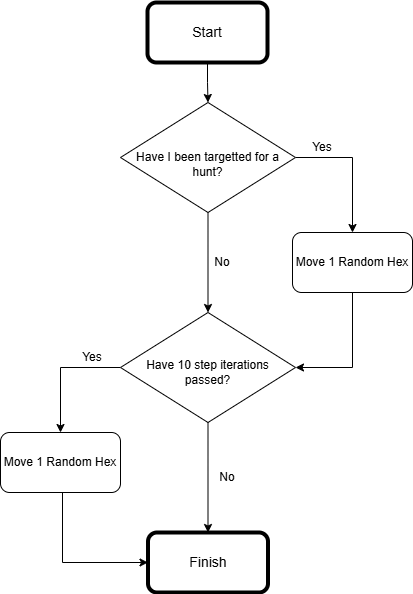
\includegraphics[width=0.5\textwidth]{PreyActionCycle.png}
		\caption{Prey Action Cycle Flowchart.}
		\label{fig:prey_action_cycle}
	\end{figure}
	  
	\section{Predator Agents}
	
	Predator agents are the active operators in this simulation. They move and hunt prey solo or in groups. They achieve the latter through negotiation with other predators in iterative bargaining rounds of temporary coalition formations. \\
	
	\textbf{Reward Function} \\
	
	Every predator $i$ operates as a rational, utility maximizer within a Probabilistic Resource-Bounded Alternating-time Temporal Logic (pRB-ATL) framework \cite{Nguyen2023}. At any discrete time step, a predator evaluating a hunting action targeting local prey $a$ calculates its expected net capture reward $\mathbb{E}[R_i(a)]$ defined as: \\
	
	\begin{equation} \label{eq:exp_hunt_utility}
		\mathbb{E}[R_i(a)] = P_{capture,i}(a) \cdot \left( x_i \cdot R_a \right) - C_{\text{hunt},i} \\
	\end{equation}
	
	where:
	\begin{itemize}
		\item $R_a$ represents the total reward gain from the target prey type $a \in \{\text{Hare}, \text{Stag}, \text{Mammoth}\}$.
		\item $P_{capture,i}(a) \in [0, 1]$ is the capture success probability (detailed in Section 3.3.3)
		\item $C_{\text{hunt},i}$ is the energy cost required during hunt execution, incurred regardless of whether the hunt succeeds or fails.
		\item $x_i \in (0, 1]$ denotes predator $i$'s proportional share of the captured reward, whether if he hunts solo or in a coalition $C$ of predators:
		\begin{equation} \label{eq:proposed_share}
			x_i = \begin{cases} 
				1.0 & \text{if } |C| = 1 \text{ (Solo Hunt)} \\[4pt]
				x_{prop, i} & \text{if } |C| > 1 \text{ (Coalition Hunt)} 
			\end{cases}
		\end{equation}
	\end{itemize}
	
	In a coalition hunt ($|C| > 1$), the share $x_{prop, i}$ is not a fixed global constant. However, it is dynamically proposed by the coalition initiator based on the active reward distribution tactic (detailed in Section 3.4.2). \\
	
	Having established the unified reward metric, in this section we also present our predator types with their respected parameters and lay the groundwork for our predators' decision-making and action execution cycle.
	
	\subsection{Predator Types}
	
	Each Predator $i$ is defined by a tuple of a fixed type vector $t_{i}$ that compromises its characteristics in a hunt scenario and by its Food stockpile $F_{i}$ that acts as an energy reserve. Besides that, they are identical in how they move or how they interact with other agents. At every simulated episode setup, each predator agent is assigned a specific type. This is not random but hard-coded so that each simulation episode loop has consistent predator types for cross-reference. Then, depending on this type, the rest of the parameters are assigned automatically:
	
	\[{Predator}_i = \langle t_i, F_{i} \rangle\]
	\[t_i = [Type_{i}, M_{i}, D_{base,i} , C_{hunt,i}] \] \\
	
	\begin{itemize}
		\item The "Baseline" represents a default type agent with basic amounts of merit, baseline demand and hunting cost. Every type's parameters are adjusted relative to this type.
		
		\item The "Specialist" represents a knowledgeable high-skill agent, with the highest merit and hunting cost out of all types, with slightly increased baseline demand.
		
		\item The "Freeloader" represents a low effort but high expectations agent, with the highest baseline demand out of all types, but with low merit and hunting effort. 
		
		\item The "Newbie" represents an inexperienced agent, with the lowest merit, baseline demand and hunting cost, being a type that offers no significant advantage but also not demanding a lot. \\  
	\end{itemize}
	
	\begin{table}[H]
		\centering
		\begin{tabular}{|c|c|c|c|}
			\hline
			$Type_{i}$ & $M_{i}$ & $D_{base,i}$ & $C_{hunt,i}$ \\
			\hline
			"Baseline" & 1.5 & 0.15 & 5.0 \\
			"Specialist" & 3.0 & 0.25 & 15.0 \\
			"Freeloader" & 0.8 & 0.4 & 3.0 \\
			"Newbie" & 0.5 & 0.05 & 1.5 \\
			\hline
		\end{tabular}
		\caption{Predator Agent Types and Parameters}
	\end{table}
	
	\textbf{Merit $M_{i}$ (Skill)} \\
	
	It represents the contribution of the predator in a hunt, acting as a multiplying factor in the hunt success probability. In this ecology, it is the individual value that the predator offers actively. In a coalition, multiple predators' merits are additive, but with diminishing returns.\\
	
	\textbf{Baseline Demand $D_{base,i}$ (Greed)} \\
	
	It represents the basic intrinsic demand percentage the predator thinks it deserves. It is the basis for the effective demand factor $D_{eff,i}$ (Eq.~\ref{eq:effective_demand_factor}), that is, depending on its remaining food stockpile, the dynamic criteria for a predator to accept a coalition proposal. \\
	
	\textbf{Hunting Cost $C_{hunt,i}$ (Effort)} \\
	
	It represents the metabolic cost to perform a hunt action. \\
	
	\textbf{Food Stockpile $F_{i}$ (Energy Reserve)} \\
	
	It represents the energy reserves of the predator. Successfully capturing prey rewards replenishes it while actions depletes it. If by any chance the stockpile reaches 0, the predators dies and cannot act anymore. The food stockpile provides the a dynamic factor to the environment that plays a crucial role in how predators decide and act. \\
	
	To evaluate the efficiency of coalition formation in a heterogeneous environment, we implement a Capacity-Constraint Agent Architecture. Each predator's parameters lie within a bounded constant $K$, preventing the emergence of "super predators", forcing the system to rely on the distribution tactics to incentivise cooperation. Formally, this architecture is based in Probabilistic Resource Bounded Alternating time Temporal Logic (PRB-ATL) \cite{Nguyen2023}. In this framework, the success of an agent is not merely a matter of strategy, but is also strictly connected to its resource budget $b$ (represented here by $K$). By bounding K, we ensure that certain high utility states are off-limits for a single predator (solo hunting Mammoth), while remaining viable for a coalition. \\
	
	\subsection{Predator's Action Cycle}
	
	At the start of each simulation step, predators perform an initial observation of all agents residing within the same Hex coordinates. Based on these observations, they update their available actions and they choose the action that maximize their expected utility gain for that time step. The resulted Decision state representation at the end of the decision phase is then processed in the execution phase. Since this process is executed linearly, all active predators are first shuffled at random and all finish their decision-making before they head to the execution. \\
	
	\textbf{The Decision Phase} \\
	
	Firstly, Resting and Moving around the coordinates are treated as default options of any predator, ensuring that they always possess a baseline behavior. Then, according to other agents' presence, hunting Solo or in Coalitions are also available. Predators can only hunt prey that hasn't already been targeted in this time-step to avoid collisions in logic. Every option is then followed by a computation function that informs the predator about its expected utility gain and the structural data necessary to execute it. 
	
	\begin{figure}[H]
		\centering
		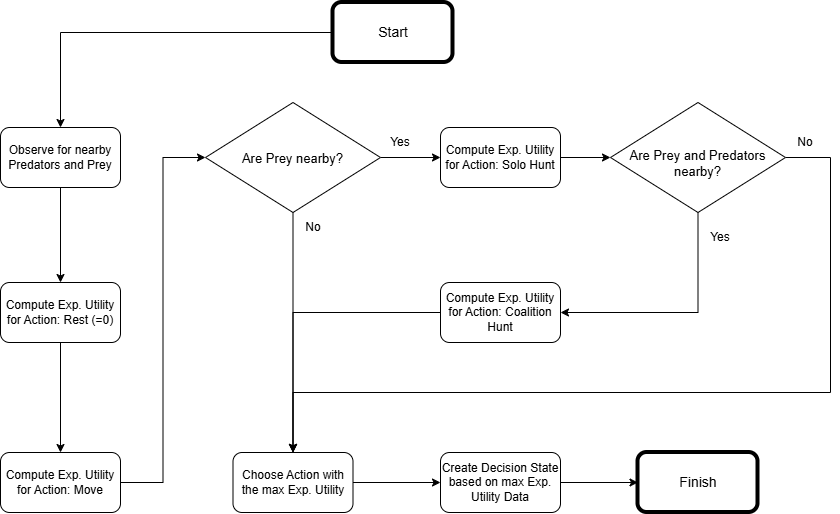
\includegraphics[width=0.7\textwidth]{DecisionPhaseCycle.png}
		\caption{Predator Decision Cycle Flowchart.}
		\label{fig:predator_decision_cycle}
	\end{figure}
	
	\textbf{Solo and Coalition Hunt} \\
	
	From now on, we define "capture" as a successful hunting attempt. For a hunting action, the probability of capturing prey $a$, for a single predator $i$ or for a coalition $C$ of predators $j$, is defined as: \\ 
	
	\begin{equation} \label{eq:p_capture}
		P_{capture}(C, a) = 1 - (1 - P_{solo}(a))^{E_{C} \cdot β_{C}}
	\end{equation}
	
	\vspace{1em}
	
	where $E_C$ is the collective effectiveness of all predators as the sum of their merits $M_j$ (Section 3.3.1) and $β_{C}$ is the synergy factor that translates to how well they coordinate to capture a specific prey $a$ (Section 3.2.1): \\
	
	\begin{equation} \label{eq:collective_eff}
		E_C =
		\begin{cases}
			\displaystyle \sum_{j \in C} M_j & \text{,if } |C| > 1 \\
			M_i & \text{,if } |C| = 1
		\end{cases}
	\end{equation}
	
	: \\
	\begin{equation}
		β_{C} =
		\begin{cases}
			β_a & \text{,if } |C| > 1 \\
			1 & \text{,if } |C| = 1
		\end{cases}
	\end{equation}
	
	\vspace{1em}
	
	As $E_{C}$ and $β_{C}$ grow, the capture probability increases. However, this function is grounded in the property of submodularity \cite{Bach2013} and its diminishing marginal returns. As coalition size increases, the utility of additional effectiveness $E_{C}$ eventually flattens out. This mathematical structure is principled because it prevents predators from simply maximizing their numbers, to instead forcing them to evaluate the marginal utility of a feasible coalition. Predators will reject a hunt proposal if the cost of participation outweighs the shrinking gains in capture probability. \\
	
	Calculating the expected utility for both solo and coalition hunting follow the same principle. For each prey in the same hex coordinates, the predator calculates its success probability $P_{capture,solo}$ (Eq.~\ref{eq:p_capture}) and the expected utility $E[U_{solo}]$ (Eq.~\ref{eq:exp_hunt_utility}) of capturing that prey. The highest reward yielding target gets chosen for the hunt. \\
	
	The difference between the hunting options lie in the other predators present. Since the coalition negotiation process lies in the execution phase, the deciding predator computes its coalition hunt expected utility by assuming all predators present are potential partners that contribute to the collective effectiveness (Eq.~\ref{eq:collective_eff}) and hunt success, taking only a specific share $x_i$ (Eq.~\ref{eq:proposed_share})  of the reward based on the active distribution tactic. If a target is chosen, a decision state representation is informed with the action chosen, a prey target, potential partners and coalition share if necessary. \\
	
	\begin{algorithm}[H]
		
		\caption{Expected Utility Calculation for Solo Hunt Action}
		\label{alg:Action_SOLO_HUNT_utility}
		
		\SetKwInput{KwIn}{Input}
		\SetKwInput{KwOut}{Output}
		
		\KwIn{predator $i$, prey present}
		\KwOut{Predator's best utility and its target prey}
		
		\BlankLine
		
		set best utility = $-\infty$\;
		set target prey = None\;
		
		\For{each prey in prey present}{
			compute solo $P_{capture,solo}$ for that prey\;
			compute solo expected utility $E[U_{solo}]$ for that prey\;
			
			\If{$E[U_{solo}]$ $>=$ best utility}{
				set best utility =  $E[U_{solo}]$\;
				set this as new target prey\;
			}
		}
	\end{algorithm}
	
	\begin{algorithm}[H]
		
		\caption{Expected Utility Calculation for Coalition Hunt Action}
		\label{alg:Action_COALITION_HUNT_utility}
		
		\SetKwInput{KwIn}{Input}
		\SetKwInput{KwOut}{Output}
		
		\KwIn{predator $i$, prey present, predators present}
		\KwOut{Predator's best utility, its target prey, its coalition share and potential partners}
		
		\BlankLine
		
		set best utility = $-\infty$\;
		set target prey = None\;
		
		set coalition C = [initiator, predators present]\;
		compute and set reward shares to each coalition predator\;
		
		\For{each prey in prey present}{
			compute group $P_{capture,C}$ for that prey\;
			compute solo expected utility $E[U_{solo}]$ for that prey, with predator's $i$ share and $P_{capture,C}$\;
			
			\If{$E[U_{solo}]$ $>=$ best utility}{
				set best utility =  $E[U_{solo}]$\;
				set this as new target prey\;
				set potential partners = predators present\;
				set predator's share = its coalition share\;
			}
		}
	\end{algorithm}
	
	\vspace{1em}
	
	\textbf{Resting and Moving} \\

	Resting is a reset action that has $E[U_{solo}] = 0$. Predators that have no viable options simply stay idle and wait for more favorable conditions. Movement is available only in the neighboring hexes of the predators. Since it is penalizing to their food stockpile with a global metabolic cost of $C_move = 5$, the expected utility of movement is always negative, resulting in constant idleness. So, there was a need for a utility calculation function that drives predators to exploration if prey was not nearby. \\
	
	For these reasons, we come up with a discounted, myopic, forward-looking expected utility function for movement. The predator evaluates each candidate neighboring hex not by its immediate payoff, but by the best discounted opportunity it opens up, that is the highest expected utility obtainable from any prey in the environment, weighted by how many further movement steps would be required to reach it. A prey in a distance of $d$ hexes away contributes a discounted reward of $γ^d*U_{solo}$, offset by the discounted cumulative cost of the $d$ steps needed to reach its coordinates. This allows a neighboring hex that moves the predator closer to a distant but valuable prey target to score some positive net utility, even though no capture is possible in this turn. This works as long as the discounted future reward outweighs the discounted cost of the journey. \\
	
	This function serves two purposes. First, it gives predators a principled reason to explore rather than remain passive. Second, it biases exploration as predators select the neighboring hex that maximizes discounted proximity to the most rewarding prey currently known, producing search behavior that resembles goal-directed foraging rather than purposeless roaming. Only when no prey exists within a horizon where $γ^d*U_{solo}$ can exceed the discounted cost of reaching it does resting again becomes the dominant action, allowing predators to conserve their food reserves stockpile until conditions improve.
	
	\begin{algorithm}[H]
		
		\caption{Expected Utility Calculation for Move Action}
		\label{alg:Action_MOVE_utility}
		
		\SetKwInput{KwIn}{Input}
		\SetKwInput{KwOut}{Output}
		
		\KwIn{predator $i$, neighboring hexes of predator $i$}
		\KwOut{Predator's best move utility, its target hex}
		
		\BlankLine
		
		set discount factor $\gamma = 0.9$\;
		set best move utility = $-\infty$\;
		set best hex = predator's current hex\;
		
		\For{each prey type $\tau$}{
			compute solo capture probability $P_{capture,i}$ for that type, with predator $i$'s hunting skill\;
			compute solo expected utility $E[U_{solo,\tau}]$ for that type, using $P_{capture,i}$\;
		}
		
		\For{each neighboring hex $h'$}{
			set best discounted value $V^{*}$ = $-\infty$\;
			
			\For{each prey in the simulation}{
				retrieve precomputed $E[U_{solo,\tau}]$ for that prey's type\;
				compute hex distance $d$ between $h'$ and that prey\;
				
				\eIf{$d = 0$}{
					set discounted value $V(h' \mid prey)$ = $E[U_{solo,\tau}]$\;
				}{
					compute discounted reward = $\gamma^{d} \cdot E[U_{solo,\tau}]$\;
					compute discounted cumulative cost = $C_{move} \cdot \dfrac{1-\gamma^{d}}{1-\gamma}$\;
					set $V(h' \mid prey)$ = discounted reward $-$ discounted cumulative cost\;
				}
				
				\If{$V(h' \mid prey) > V^{*}$}{
					set $V^{*}$ = $V(h' \mid prey)$\;
				}
			}
			
			compute move utility for $h'$ = $-C_{move} + \gamma \cdot V^{*}$\;
			
			\If{move utility for $h'$ $>$ best move utility}{
				set best move utility = move utility for $h'$\;
				set best hex = $h'$\;
			}
		}
	\end{algorithm}
	
	\vspace{1em}
	
	\textbf{The Execution Phase} \\
	
	Once every predator passes through the decision phase, each one acts according to their decision state representation. Moving predators travel to the specified hex coordinates deemed most valuable. Hunting predators either hunt their target prey immediately or they pass through the coalition negotiation process first. This deems who of the potential partners actually form a coalition with the active predator and hunt the prey together. The formation framework is further explained in Section 3.4. Hunting is probabilistic, and the predator is rewarded its actual utility if the hunt is successful, or it is penalized with his hunting effort.
	
	\begin{figure}[H]
		\centering
		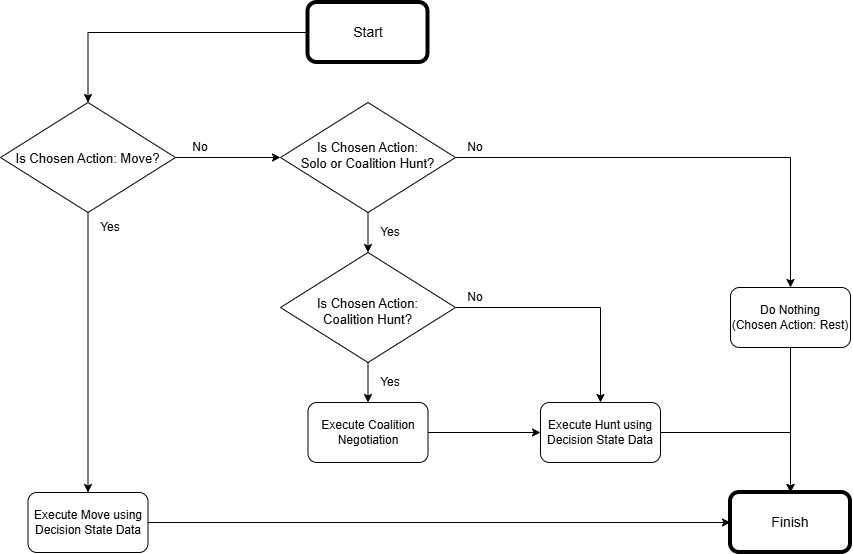
\includegraphics[width=0.7\textwidth]{ExecutionPhaseCycle.png}
		\caption{Predator Execution Cycle Flowchart.}
		\label{fig:predator_execution_cycle}
	\end{figure}
	
	\section{Coalitional Formation Framework}
	
	Once a Coalition Hunt action is chosen, the initiator goes through the negotiation process that will determine if the predators close to it can actually come to an agreement, forming a temporary coalition to hunt the targeted prey as a group.
	
	\subsection{Iterative Bargaining Protocol}
	
	The actual formation of that coalition is resolved through an Iterative Bargaining Protocol. The initiator begins with all nearby predators in the same hex as its pool of potential partners and proposes a coalition $C$ consisting of itself and this entire pool. For this proposed coalition, the group capture probability $P_{capture,C}$ is recomputed (Eq.~\ref{eq:p_capture}), along with the reward share owned to each potential partner$j$ according to the active distribution tactic (Section 3.4.2). This proposal is then evaluated independently by every predator, each of whom checks it against the two acceptance criteria established in Section 3.4.3: the bargaining check, verifying that the offered share meets or exceeds their effective demand factor (Eq.~\ref{eq:bargaining_check}), and the utility check, verifying that their expected utility under the coalition is at least as great as what they would expect from hunting solo (Eq.~\ref{eq:utility_check}). A partner must satisfy both conditions to accept the proposal. \\
	
	If every member of the proposed pool accepts, the coalition is immediately finalized as stable and the protocol terminates. However, even if a single predator rejects the proposal, the entire round is considered a failure rather than a partial success. The initiator does not negotiate individually with the remaining accepters. Instead, it removes the rejecting predators from its pool of potential partners and proposes a new, smaller coalition $C'$ to the reduced set, recomputing the group capture probability and reward shares to reflect this new composition. This shrinking continues iteratively, giving every remaining partner a fresh opportunity to accept or reject the recalculated terms, until either a fully accepting subset is found or the pool of potential partners is exhausted entirely. \\
	
	If the latter happens, the initiator abandons the coalition attempt altogether and falls back to hunting solo, updating its own decision state with a recalculated solo capture probability and a full reward share of $x_i = 1.0$. This outcome mirrors the notion of involuntary unemployment in coalitional bargaining theory:. The initiator is not prevented from hunting, but is denied the cooperative gains that a successful coalition would have offered. Furthermore, once a stable coalition $C'$ is reached, every one of its members has their decision state updated to reflect a Coalition Hunt action, tagged with their finalized reward share and the group's capture probability, and is marked as having acted for this time-step to prevent it from being reconsidered by any other initiator's negotiation in the same round. \\ 
	
	\begin{algorithm}[H]
		\caption{Iterative Coalition Bargaining Protocol}
		\label{alg:execute_coalition_negotiation}
		
		\SetKwInput{KwIn}{Input}
		\SetKwInput{KwOut}{Output}
		
		\KwIn{Initiator agent $i$, Target prey $y$}
		\KwOut{Updated decision states and reward shares for all active predators}
		
		\BlankLine
		
		set current partners = initiator's nearby predators\;
		
		\While{true}{
			set coalition C = [initiator, current partners]\;
			compute group $P_{capture,C}$ for target prey $y$\;
			compute and set reward shares to each coalition predator\;
			
			\For{each partner in current partners}{
				get partner's coalition checks\;
			}
			
			\If{all partners accepted}{
				\textbf{break} loop\;
			}
			
			\If{no partners accepted}{
				assign "Solo Hunt" to initiator action state\;
				update initiator decision state with new solo $P_{capture, i}$ and reward share = 1.0\;
				\Return\;
			}
			\Else{
				shrink current partners to accepted partners\;
			}
		}
		set stable coalition C' = [initiator, current partners]\;
		\For{each predator in stable coalition C'}{
			assign "Coalition Hunt" to predator's action state\;
			assign calculated reward share and group $P_{capture,C'}$  to predator\;
			mark predator as acted\;
			update predator's decision state;
		}
	\end{algorithm}
	
	\vspace{1em}
	
	This structure follows the random-proposer model of coalitional bargaining \cite{Okada2011}, in which a single proposer dictates both the composition of the coalition and the allocation of its surplus, and potential partners respond only by accepting or rejecting the offer as given rather than counter-proposing. The two-check acceptance criterion corresponds to the discounted payoff threshold that a responder requires in a stationary sub-game perfect equilibrium (SSPE) \cite{Okada2011} in order to rationally accept a proposal rather than hold out for a better one. Because the protocol is non-negotiable and one-way, it deliberately sacrifices the full generality of iterative counter-offer bargaining in exchange for computational tractability, while still preserving the core game-theoretic property that only mutually rational, individually improving coalitions are ever allowed to form.
		
	\subsection{Reward Distribution Tactics}

	To analyze the impact of different resource sharing strategies on predator efficiency and coalition feasibility, we implement four, distinct reward distribution tactics based on established principles of distributive justice in Multi-Agent Systems \cite{Deutsch1975}. \\
	
	\textbf{Egalitarian:} The Fair-based split. In this tactic, the captured reward is distributed equally among the predators $j$ of the coalition $C$. For a split share $x_{prop,i}$ of a predator $i$: \\
	
	\[ x_{prop,i} = \frac{1}{|C|} \] \\
	
	\textbf{Meritocratic:} The Skill-based split. In this tactic, the captured reward is distributed proportionally to each predator's contribution (merit). Each predator $i$ receives a share relative to its merit $M_i$ compared to the total merit of all predators $j$ in the coalition $C$: \\
	
	\[ x_{prop,i} = \frac{M_i}{\sum_{j \in C} M_j} \] \\
	
	\textbf{Altruistic:} The Need-based split. In this tactic, the captured reward is distributed proportionally to each predator's Effective Demand Factor $D_{eff,i}$, as proposed in section 3.4.3, relative to the total $D_{eff,j}$ of all predators $j$ in the coalition $C$. Predators with higher energetic need receive a larger share of the reward: \\
	
	\[ x_{prop,i} = \frac{D_{\text{eff},i}}{\sum_{j \in C} D_{\text{eff},j}} \] \\
	
	\textbf{Asymmetric:} The Leader's share split. This tactic is based on the concept that realistic coalition formation compensates the proposer for its effort and coordination \cite{Chalkiadakis2011}. Thus, the initiator of the hunt receives a fixed share of the reward, while the remaining reward is equally distributed among all members of the coalition. The leader's share is currently at $L = 0.2$ for testing purposes and can be changed globally at the start of the simulation. Each predator $i$ receives: \\
	
	\[
	x_{\text{prop},i} =
	\begin{cases}
		L + \dfrac{1 - L}{|C|} & \text{if } i \text{ is the initiator} \\ \\
		\dfrac{1 - L}{|C|} & \text{if } i \text{ is a partner}
	\end{cases}
	\] 
	
	\subsection{Proposal Acceptance Criteria (EDF)}
	
	In order to understand how predators evaluate a coalition proposal, first we need to introduce the Effective Demand Factor $D_{eff,i}$. It is the current, non-negotiable, threshold percentage of the reward that the predator must be offered to participate in this coalition hunt. It is dynamic, driven by the predator's baseline demand that is amplified by a factor relative to his remaining food stockpile and hunting cost. It represents his actual desperation for gain relative to the imminent hunting action and his current food stockpile: \\
	
	\begin{equation} \label{eq:effective_demand_factor}
		D_{eff,i}(F_{i}) = D_{base,i} \cdot [1 + e^{-F_{i} / C_{hunt,i}}] \\
	\end{equation}
	
	\vspace{1em}
	
	Each potential partner $j$ in a coalition negotiation goes through two distinct evaluations: the Bargaining and Utility checks respectively. The bargaining check refers to whether the proposed share for that partner is greater than its effective demand factor, translating to "does this hunt exceeds my dynamic expectations of what I think I deserve?" and the utility check refers to whether the expected utility for this coalition hunt with this proposed share is greater than the supposed expected utility if that predator was hunting solo, translating to "Is this coalition hunt more beneficial for me than hunting solo?" Both of these evaluations have to pass for the potential partner $j$ to be a part of this coalition. For computation reasons, once it fails the bargaining check, the predator never passes through the utility check: \\
	
	\begin{equation}\label{eq:bargaining_check}
		x_{prop,j} \geq D_{eff,j}
	\end{equation}
	
	\vspace{1em}
	
	\begin{equation} \label{eq:utility_check}
		E[U_{group}] \geq E[U_{solo}]
	\end{equation}
	
	 where,
	
	\[ E[U_{group}] = P_{capture, group} \cdot (x_{prop,j} \cdot R_{a}) - C_{hunt,j} \]
	
	\[ E[U_{solo}] = P_{capture, solo} \cdot R_{a} - C_{hunt,j} \]
	
	\vspace{1em}
	
	\chapter{Experiments and Results}
	\label{ch:simulations}
	In this chapter, we use the simulation environment we built to compare the performance of our distribution tactics from Section 3.4.2, using various types of predators.The first experiment features a homogeneous predator population with normal synergistic bonus, while the second and third experiments feature a heterogeneous predator population with normal and high synergistic bonus respectively. \\
	
	For the evaluation and comparison, we measure the average hunt performance and utility distribution from the predators' type interactions with a 0.95 confidence interval across the entirety of seeded episodes. These include the total of solo hunt attempts and group hunt attempts under a coalition formation, while also the utility gained from hunting solo and from hunting in a coalition, either as an initiator or a partner. \\
	
	\section{Simulated Experiments}
	
	Every experiment we conduct features 10 predators and 25 prey agents for a total of 10,000 episodes, 500 time-steps each. Predator type vary across experiments while prey types are assigned at random in each episode. Furthermore, we use Seed generation to verify that the experimental results are academically justifiable. \\
	
	Every episode number acts as a unique seed of the simulation environment. In every seed, each random act is identical, including but not limited to:
	
	\begin{itemize}
		\item Agents' positions upon setup.
		\item Prey type assignment.
		\item Agent movement where randomness is required.
	\end{itemize}
	
	If the specific conditions of a hunt attempt are also identical (predator types and positions), then the hunting result will also be exact across the four tactics and the three experiments. This way, the only difference will reside in how predators decide rationally with each distribution tactic in place and not in an unfortunate sequence of events. \\  

	\subsection{Homogeneous Predators, Normal Synergy}
	
	In this experiment, we setup the most basic form of the simulation that consists of 10 "Baseline" predators, with a synergy factor of $β = 1$. Since every predator's type vector is identical, this experiment acts as a control condition, isolating the effect of the distribution tactic itself from any effect of population heterogeneity. \\
	
	As expected, solo hunting frequency is stable across all four tactics (123.2 - 124), with a minimal increase in the Asymmetric scenario. However, the symmetrical tactics (Altruistic, Egalitarian, Meritocratic) produce numerically identical coalition hunt frequency (24.64) as is a direct mathematical consequence of the split reward functions. When every predator has the same parameters and rational thresholds, the only tactic that shows a real behavioral difference is Asymmetric, bringing forth fewer coalition hunts (18.71) and a visible utility gap between initiator (340.73) and partner (290.44) roles.
	
	\begin{figure}[H]
		\centering
		\includegraphics[width=1\textwidth]{EXP_1_Baseline_10K_A.png}
		\caption{Baseline Predator - Hunting Performance (Homogeneous, Normal Synergy).}
		\label{fig:exp_1_baseline_A}
	\end{figure}
	
	\begin{figure}[H]
		\centering
		\includegraphics[width=1\textwidth]{EXP_1_Baseline_10K_B.png}
		\caption{Baseline Predator - Utility Distribution (Homogeneous, Normal Synergy).}
		\label{fig:exp_1_baseline_B}
	\end{figure}
	
	This experiment is a solid proof that the tactic itself only matters when predators are heterogeneous enough for it to differentiate their shares. No tactic provides a clear increase in cooperation. In symmetric split rules, homogeneity flattens out any difference that only the Asymmetric split with clearly defined roles can result in a slight utility advantage, that doesn't necessarily promote social welfare. \\
	
	\subsection{Heterogeneous Predators, Normal Synergy}
	
	In Experiment 2, we make the predators heterogeneous in terms of type. The setup consists of 10 predators, 2 for each unique type with a synergy factor of $β = 1$. We conclude with the following results from the average per type graphs listed below: \\
	
	\textbf{Baseline Predators}	\\
	
	Baseline predators keep a consistent solo hunt frequency. Coalition hunt frequency is also slightly reduced from the previous experiment. However, its values vary drastically between the lowest average (Altruistic, 12.21) and the highest (Meritocratic, 20.35). Under Altruistic, Baseline's modest demand leaves it a relatively smaller slice whenever paired with a genuinely needy partner, which most likely fails Baseline's own utility check, not resulting in a feasible coalition as often as other more demanding types. Under Meritocratic, Baseline's mid-tier merit is enough to get a sufficient coalition share when partnered with a Specialist. Indeed, the utility distribution figure confirms that Baseline predators earn considerably more as partners under Meritocratic than any other tactic-role combination, consistent with a strategy of joining coalitions led by higher-merit predators as the most rational choice.
	
	\begin{figure}[H]
		\centering
		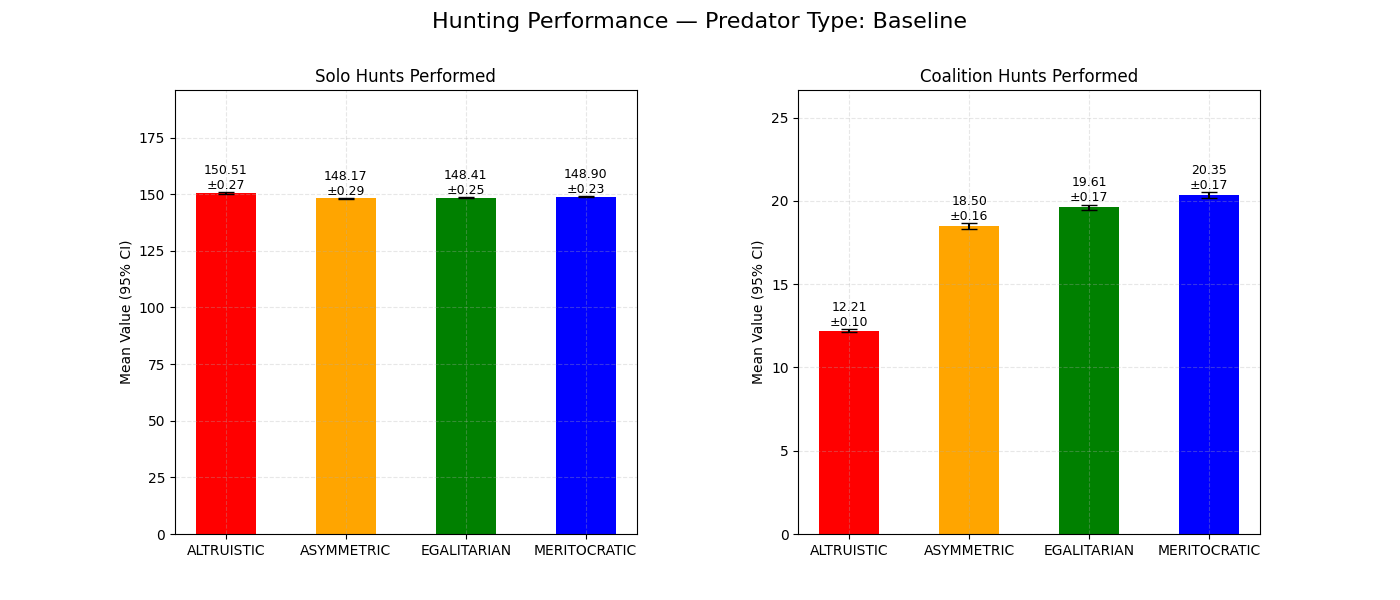
\includegraphics[width=1\textwidth]{EXP_2_BASELINE_10K_A.png}
		\caption{Baseline Predator - Hunting Performance (Heterogeneous, Normal Synergy).}
		\label{fig:exp_2_baseline_A}
	\end{figure}
	
	\begin{figure}[H]
		\centering
		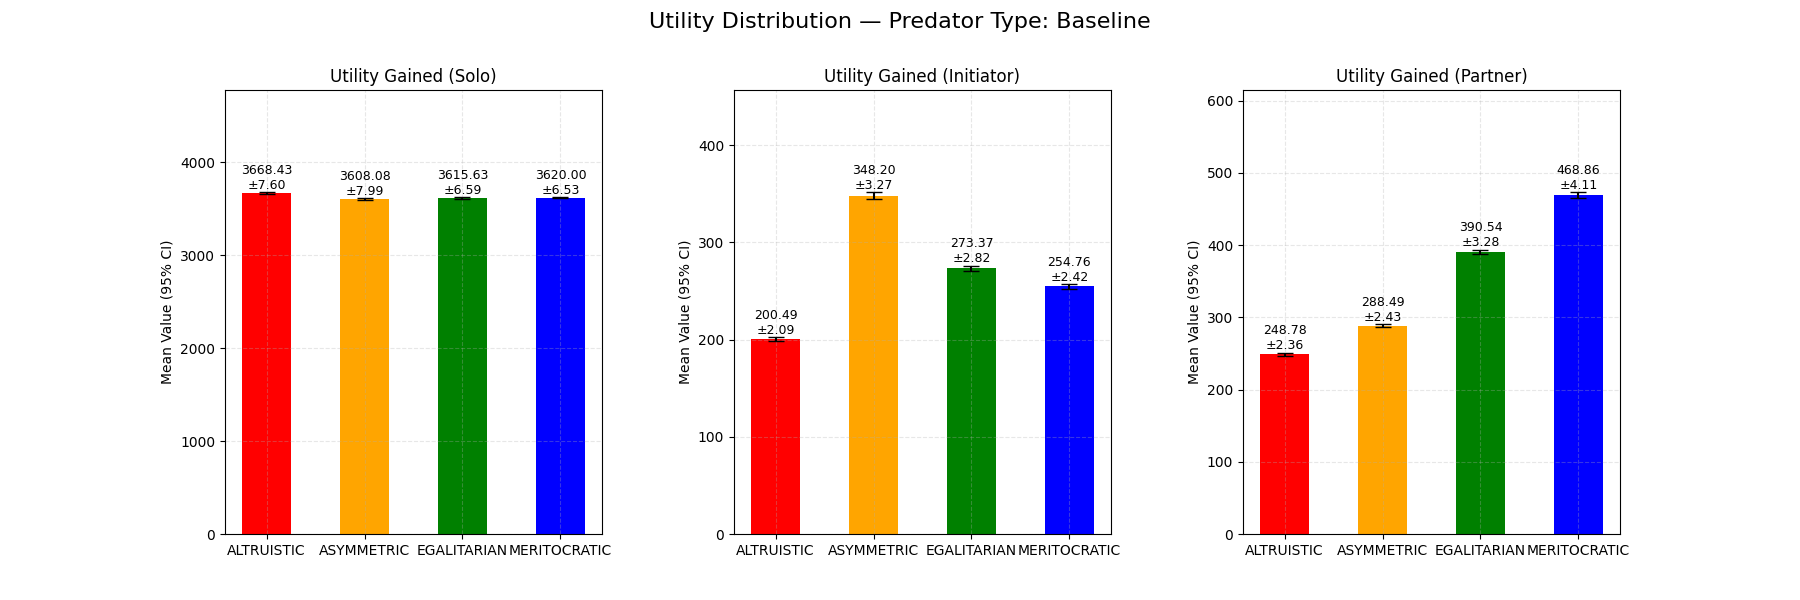
\includegraphics[width=1\textwidth]{EXP_2_BASELINE_10K_B.png}
		\caption{Baseline Predator - Utility Distribution (Heterogeneous, Normal Synergy).}
		\label{fig:exp_2_baseline_B}
	\end{figure}	
	
	\textbf{Specialist Predators} \\
	
	Specialist predators dominate with the highest solo utility gain (~4660–4707) despite the high hunting cost, and by far the highest coalition participation (57–72 hunts), three to four times of any other predator type respectively. Specialists are the least sensitive to which distribution tactic is active, since their high merit makes their bargaining position strong under all four. However, one notable asymmetry comes under Egalitarian and Meritocratic, where they earn more as a partner than as an initiator, suggesting that other types' proposals are frequently structured around recruiting a Specialist rather than the reverse. They tend not to initiate coalitions often since they can outperform them by hunting alone, effectively failing their Utility check and instead choosing to gain all the benefit of a hunt.
	
	\begin{figure}[H]
		\centering
		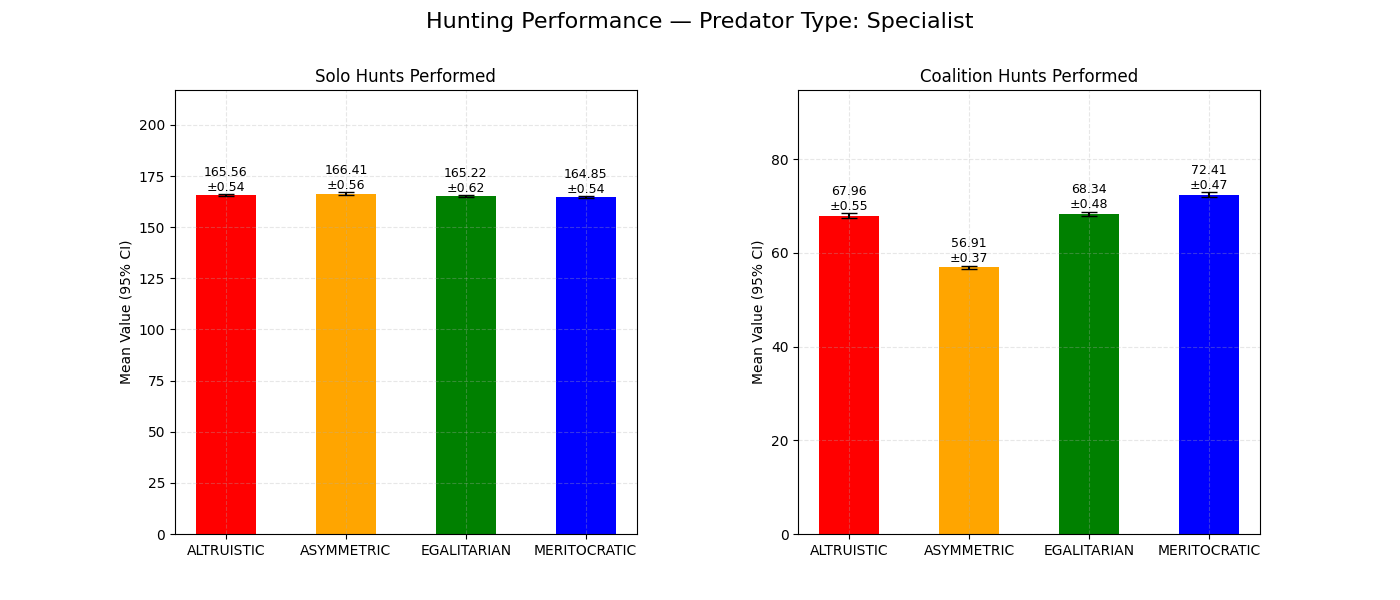
\includegraphics[width=1\textwidth]{EXP_2_SPECIALIST_10K_A.png}
		\caption{Specialist Predator - Hunting Performance (Heterogeneous, Normal Synergy).}
		\label{fig:exp_2_Specialist_A}
	\end{figure}

	\begin{figure}[H]
		\centering
		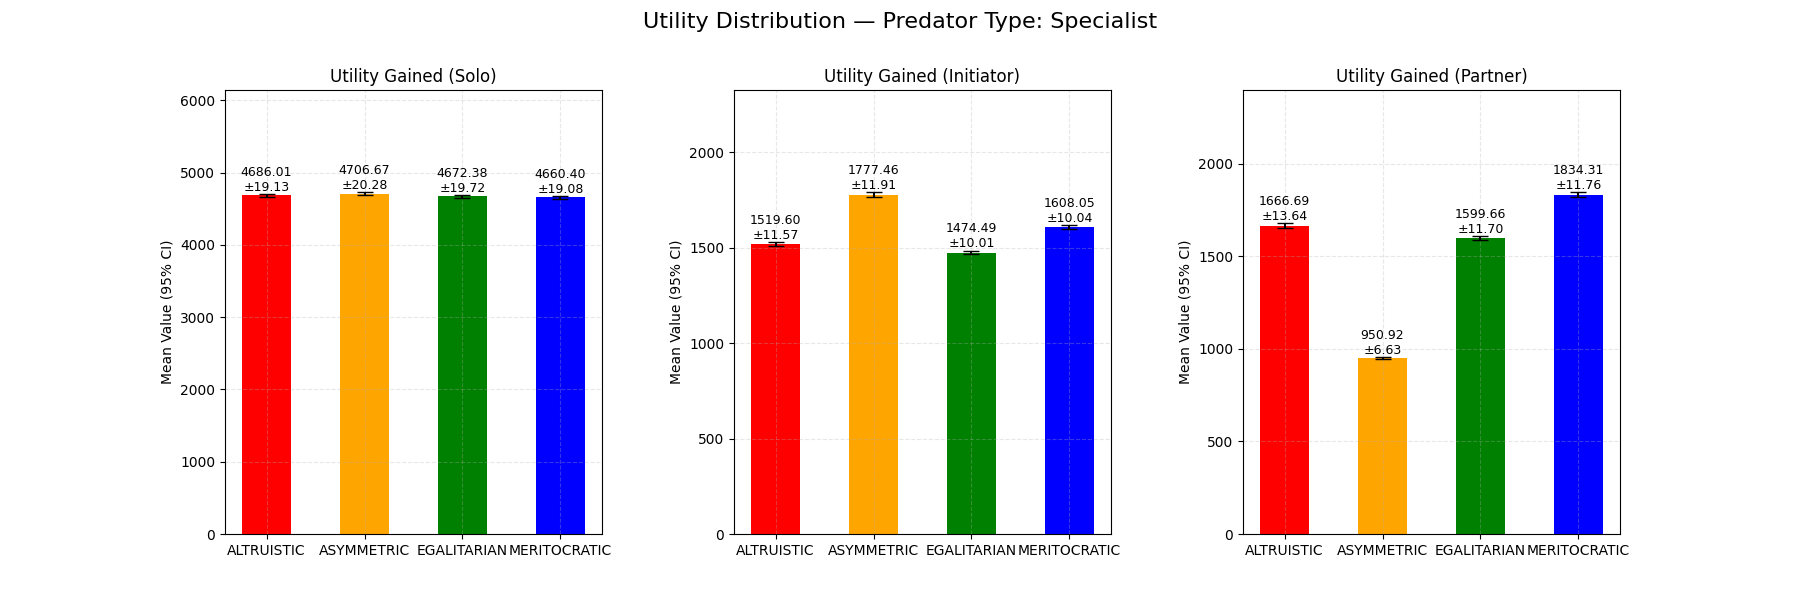
\includegraphics[width=1\textwidth]{EXP_2_SPECIALIST_10K_B.png}
		\caption{Specialist Predator - Utility Distribution (Heterogeneous, Normal Synergy).}
		\label{fig:exp_2_Specialist_B}
	\end{figure}
	
	\textbf{Freeloader Predators} \\
	
	Freeloader predators show the clearest divergence between individual and cooperative viability. Their low merit is shown in both their solo hunt frequency (135–143) and their solo utility gain (~2070–2175), while their low hunting cost keeps the bar for a profitable coalition low. This combination explains why Freeloaders are the most responsive of any type to the Meritocratic tactic (38.19 coalition hunts, nearly double Baseline's), which at first looks paradoxical for a low merit predator under contribution-based splitting. The resolution lies in the capture probability function which scales with the coalition's combined effectiveness, so a Freeloader riding alongside its potential high merit partners,  experiences a large jump in success probability even for a small contribution weighted share. Furthermore, since its hunting cost is low, even a modest expected payoff passes the utility check. This is a more accurate reading of "freeloading" than passive exploitation. It is an active, rational response from a type with low cost of participation (low hunting cost), combined with someone else doing the heavy lifting.

	\begin{figure}[H]
		\centering
		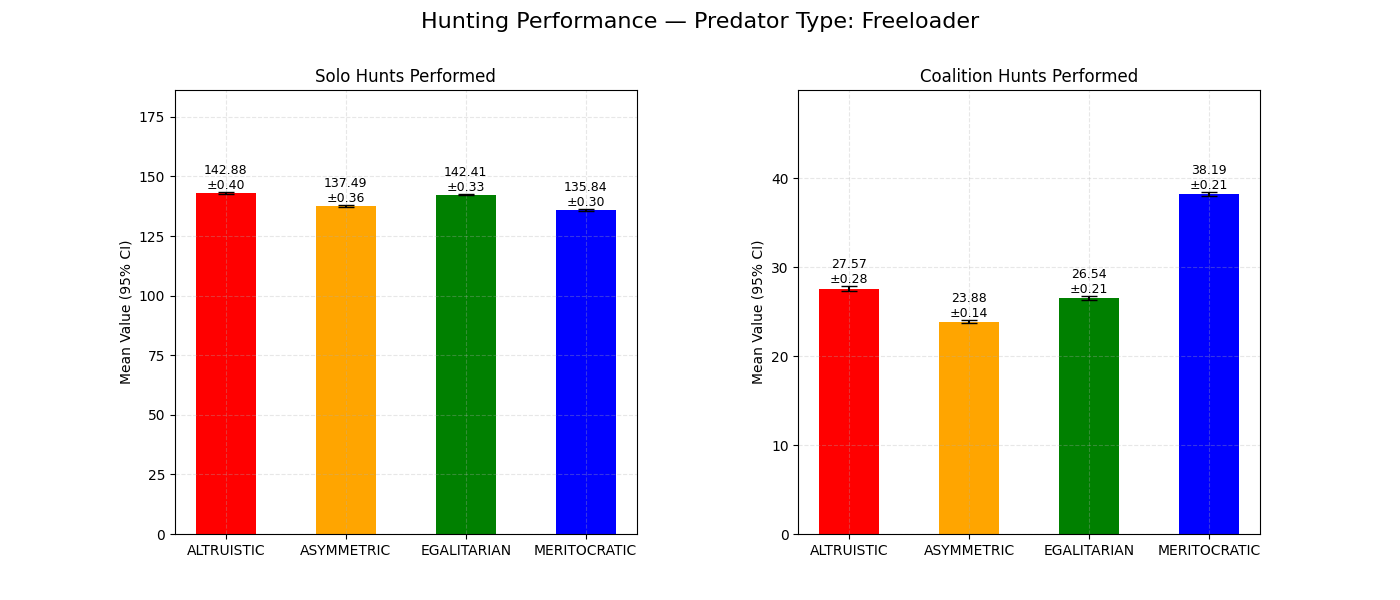
\includegraphics[width=1\textwidth]{EXP_2_FREELOADER_10K_A.png}
		\caption{Freeloader Predator - Hunting Performance (Heterogeneous, Normal Synergy).}
		\label{fig:exp_2_Freeloader_A}
	\end{figure}
	
	\begin{figure}[H]
		\centering
		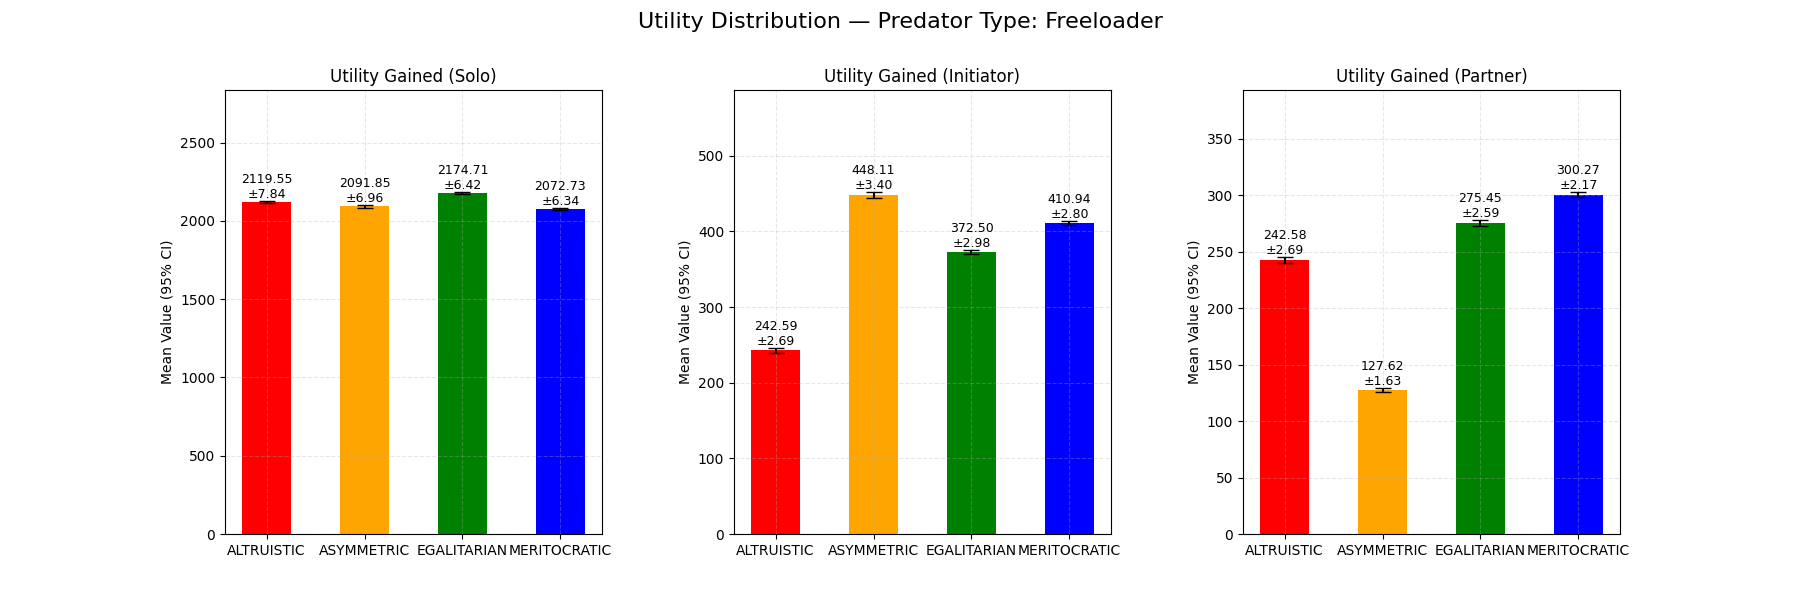
\includegraphics[width=1\textwidth]{EXP_2_FREELOADER_10K_B.png}
		\caption{Freeloader Predator - Utility Distribution (Heterogeneous, Normal Synergy).}
		\label{fig:exp_2_Freeloader_B}
	\end{figure}
	
	\textbf{Newbie Predators} \\
	
	Newbie predators' solo hunt frequency is the highest out of all types (179–193) but at roughly half of their utility yield. This is the expected outcome for a type with low merit, lowest effort cost, as the low requirement to act means Newbies attempt hunts often even when individual success odds are poor. Their near-zero base demand also produces the lowest possible bargaining threshold and they accept almost any proposed share. This explains their second highest response to Meritocratic coalitions at 40.79 hunts, the highest coalition count in the population after Specialist. They are willing partners under almost any tactic, so their coalition hunt frequency tracks whichever tactic produces the largest capture probability gain for the coalitions they're invited into, rather than which tactic gives them the largest personal share. It is important to note that Newbies earn more as partners (411.10) than initiators (138.02) under Asymmetric, the complete opposite of every other type, indicating that their low merit does not produce a high enough success chance to recruit others to get the benefit of the leader's share $L$ but are almost always recruited once someone else initiates a coalition.
	
	\begin{figure}[H]
		\centering
		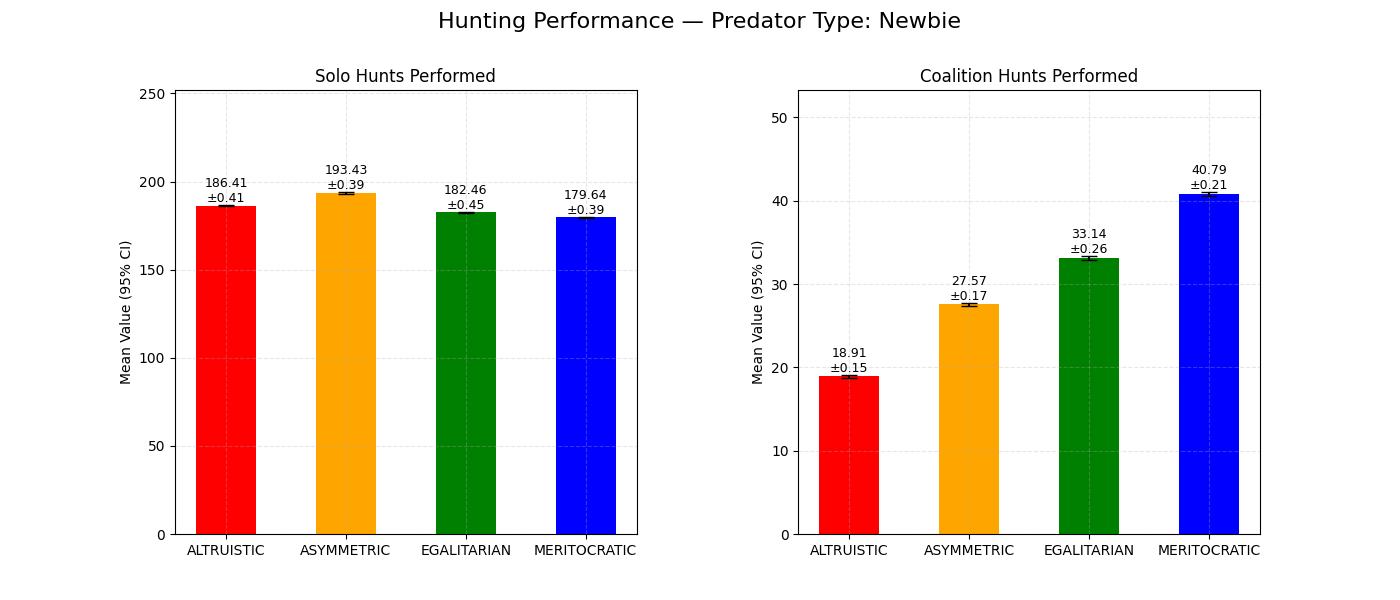
\includegraphics[width=1\textwidth]{EXP_2_NEWBIE_10K_A.png}
		\caption{Newbie Predator - Hunting Performance (Heterogeneous, Normal Synergy).}
		\label{fig:exp_2_Newbie_A}
	\end{figure}
	
	\begin{figure}[H]
		\centering
		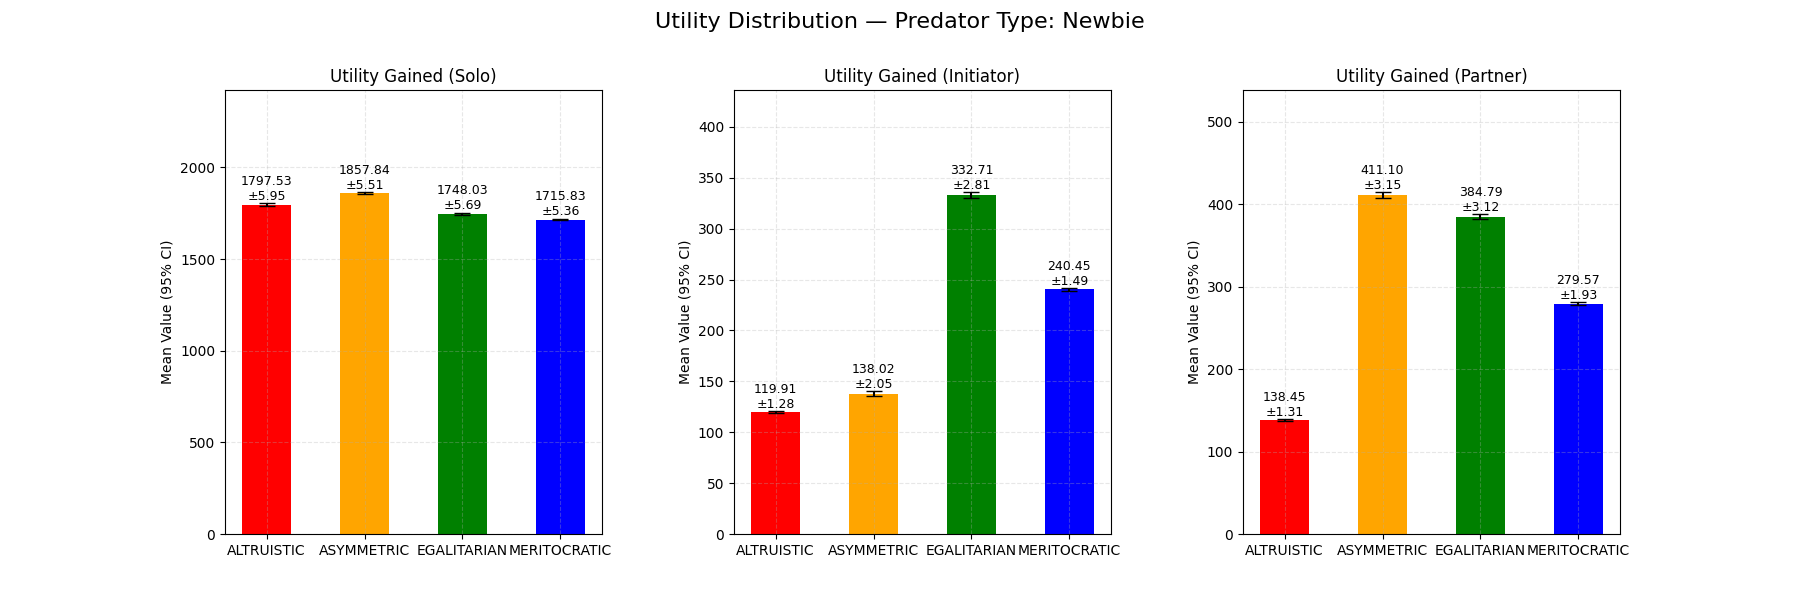
\includegraphics[width=1\textwidth]{EXP_2_NEWBIE_10K_B.png}
		\caption{Newbie Predator - Utility Distribution (Heterogeneous, Normal Synergy).}
		\label{fig:exp_2_Newbie_B}
	\end{figure} 
	
	This experiment concludes that once heterogeneity is introduced, the Meritocratic distribution tactic give the strongest cooperation incentive for every single predator type, not just on average. At first, this seems counter-intuitive for a merit based rule that should, in principle, alienate low merit predators. However, the presence of Specialists negates that disadvantage, providing that much needed success in coalition hunts when they are sought after as partners. The Egalitarian tactic is a strong second, reliably the runner-up for almost every predator, by guaranteeing every partner an unconditionally fair share regardless of merit or demand. Despite been marginally better than Asymmetric, the Altruistic tactic is the weakest overall incentive for cooperation as it has a huge variance between predator types. \\
	
	By a utilitarian standpoint, averaging the utilities gained as initiator and partner respectively, Meritocratic also produces the most utility out of all tactics and types since it is the main drive of cooperation. However, by an equity measure, Egalitarian is the fairer welfare outcome, as weak types are never squeezed into the bottom ends of the utility gain graphs the way a purely merit-blind reading of contribution would. Although, in this normal synergy setup, Meritocratic hasn't yet produced that extreme. \\
	
	\begin{table}[H]
		\centering
		\begin{tabular}{|c|c|c|c|c|c|}
			\hline
			Tactic & Baseline & Specialist & Freeloader & Newbie & Total \\
			\hline
			Altruistic & 12.21 & 67.96 & 27.57 & 18.91 & 126.65 \\
			Asymmetric & 18.50 & 56.91 & 23.88 & 27.57 & 126.86 \\
			Egalitarian & 19.61 & 68.34 & 26.54 & 33.14 & 147.63 \\
			Meritocratic & \textbf{20.35} & \textbf{72.41} & \textbf{38.19} & \textbf{40.79} & \textbf{171.74}\\
			\hline
		\end{tabular}
		\caption{Average Coalition Frequency (Heterogeneous, Normal Synergy)}
	\end{table}
	
	\begin{table}[H]
		\centering
		\begin{tabular}{|c|c|c|c|c|c|}
			\hline
			Tactic & Baseline & Specialist & Freeloader & Newbie & Total \\
			\hline
			Altruistic & 224.64 & 1593.15 & 242.59 & 129.18 & 2189.56 \\
			Asymmetric & 318.35 & 1364.19 & 287.87 & 274.56 & 2244.97 \\
			Egalitarian & 331.96 & 1537.08 & 323.98 & \textbf{358.75} & 2551.77 \\
			Meritocratic & \textbf{361.81} & \textbf{1721.18} & \textbf{355.61} & 260.01 & \textbf{2698.61}\\
			\hline
		\end{tabular}
		\caption{Average Coalition Utility (Heterogeneous, Normal Synergy)}
	\end{table}
	
	\subsection{Heterogeneous Predators, High Synergy}
	
	In Experiment 3, we differentiate from the previous iteration by simulating an environment where synergy plays a much grander role in cooperation. So, with the same setup as experiment 2 but with a synergy factor of $β = 2$, we conclude with the following results from the average per type graphs listed below: \\
	
	\textbf{Baseline Predators} \\
	
	Baseline predators show their widest tactic variance yet. Coalition hunts range from 21.62 in Egalitarian to 48.38 in Meritocratic. This is a huge difference from the first experiment's homogeneous case, where Egalitarian and Meritocratic were indistinguishable. Here, with Specialists  and Freeloaders also in the population, Meritocratic sharing lets Baseline extract much value from high merit partners while contributing relatively little in the hunt success probability itself, as Baseline earnings nearly triple for partner utility under Meritocratic (1327.00) versus Egalitarian (630.88). Egalitarian, by contrast, forces Baseline into a flat equity share regardless of who it partners with, which depresses the incentive to seek out high-synergy coalitions with Specialists specifically — hence the lowest coalition count of any tactic for this type.
	
	\begin{figure}[H]
		\centering
		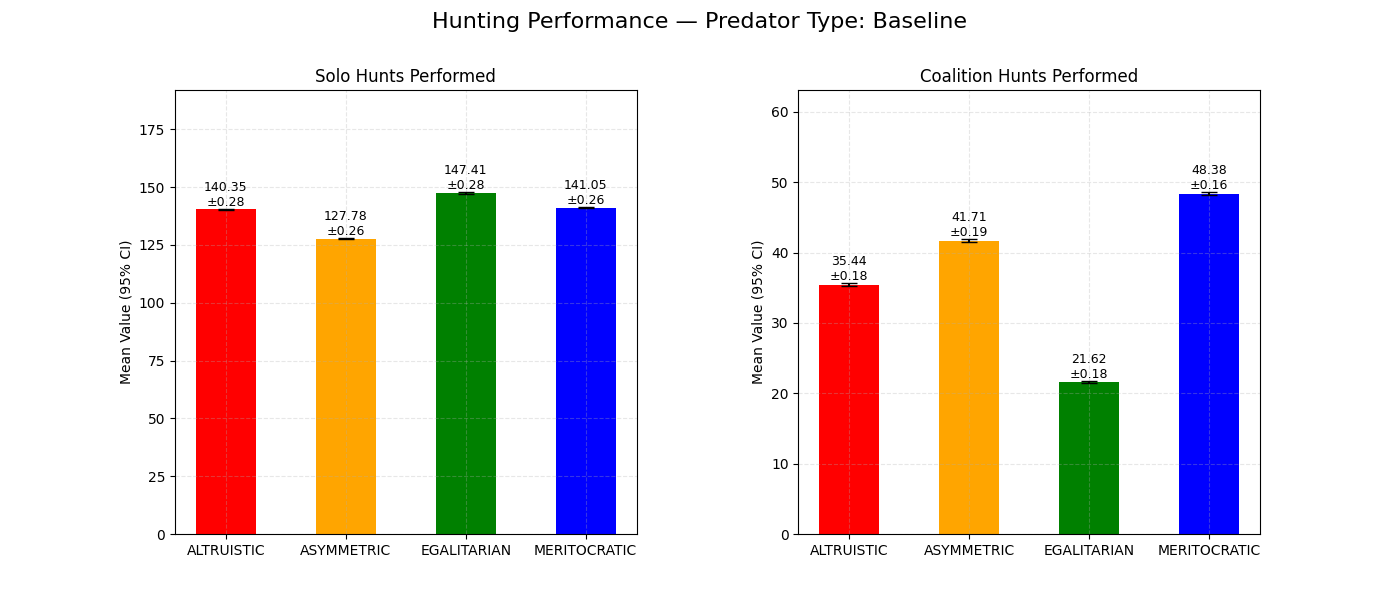
\includegraphics[width=1\textwidth]{EXP_3_BASELINE_10K_A.png}
		\caption{Baseline Predator - Hunting Performance (Heterogeneous, High Synergy).}
		\label{fig:exp_3_baseline_A}
	\end{figure}
	
	\begin{figure}[H]
		\centering
		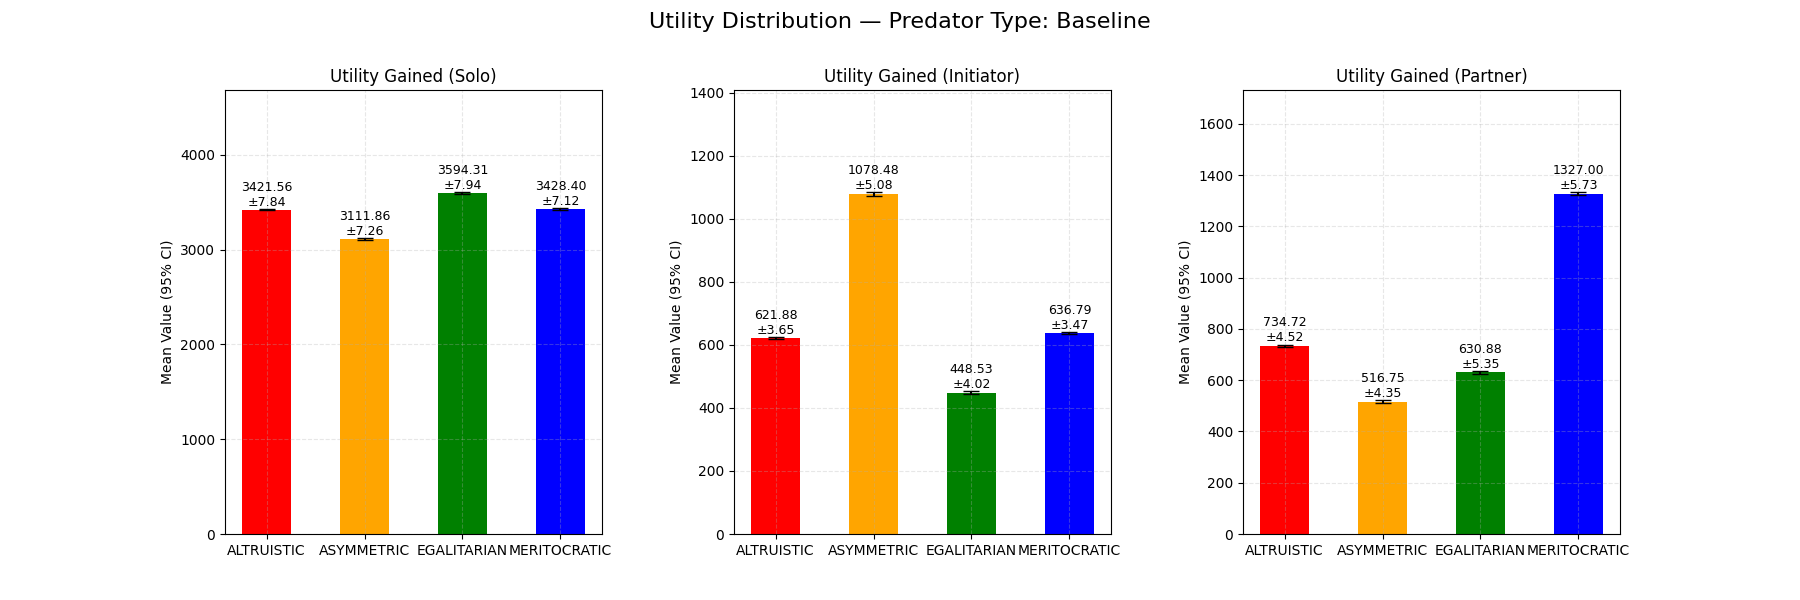
\includegraphics[width=1\textwidth]{EXP_3_BASELINE_10K_B.png}
		\caption{Baseline Predator - Utility Distribution (Heterogeneous, High Synergy).}
		\label{fig:exp_3_baseline_B}
	\end{figure}
	
	\textbf{Specialist Predators} \\
	
	Specialist predators remain the dominant type on every metric, but high synergy narrows its relative advantage over freeloader and Newbie types in coalition counts even as it widens the utility difference. Specialist's cooperative hunts are now much closer numerically as high success chances make coalition participation broadly rational for everyone, reducing the frequency variance. Despite that, Specialist's utility as partner under Meritocratic (2399.15) is nearly double to Freeloader's (461.19) or Newbie's (626.45) partner utility. This combination of coalition frequency and utility distribution asymmetry confirms that Meritocracy in a heterogeneous environment leads to elite clustering of agents, regardless of how well they cooperate.
	
	\begin{figure}[H]
		\centering
		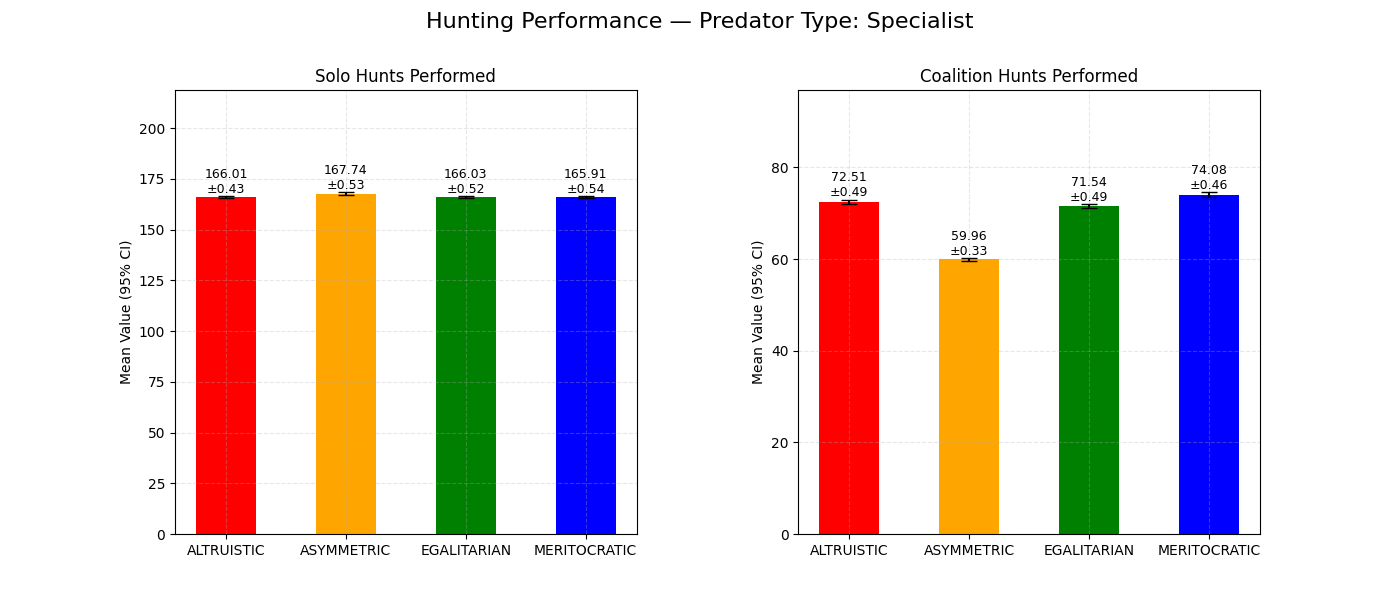
\includegraphics[width=1\textwidth]{EXP_3_SPECIALIST_10K_A.png}
		\caption{Specialist Predator - Hunting Performance (Heterogeneous, High Synergy).}
		\label{fig:exp_3_Specialist_A}
	\end{figure}
	
	\begin{figure}[H]
		\centering
		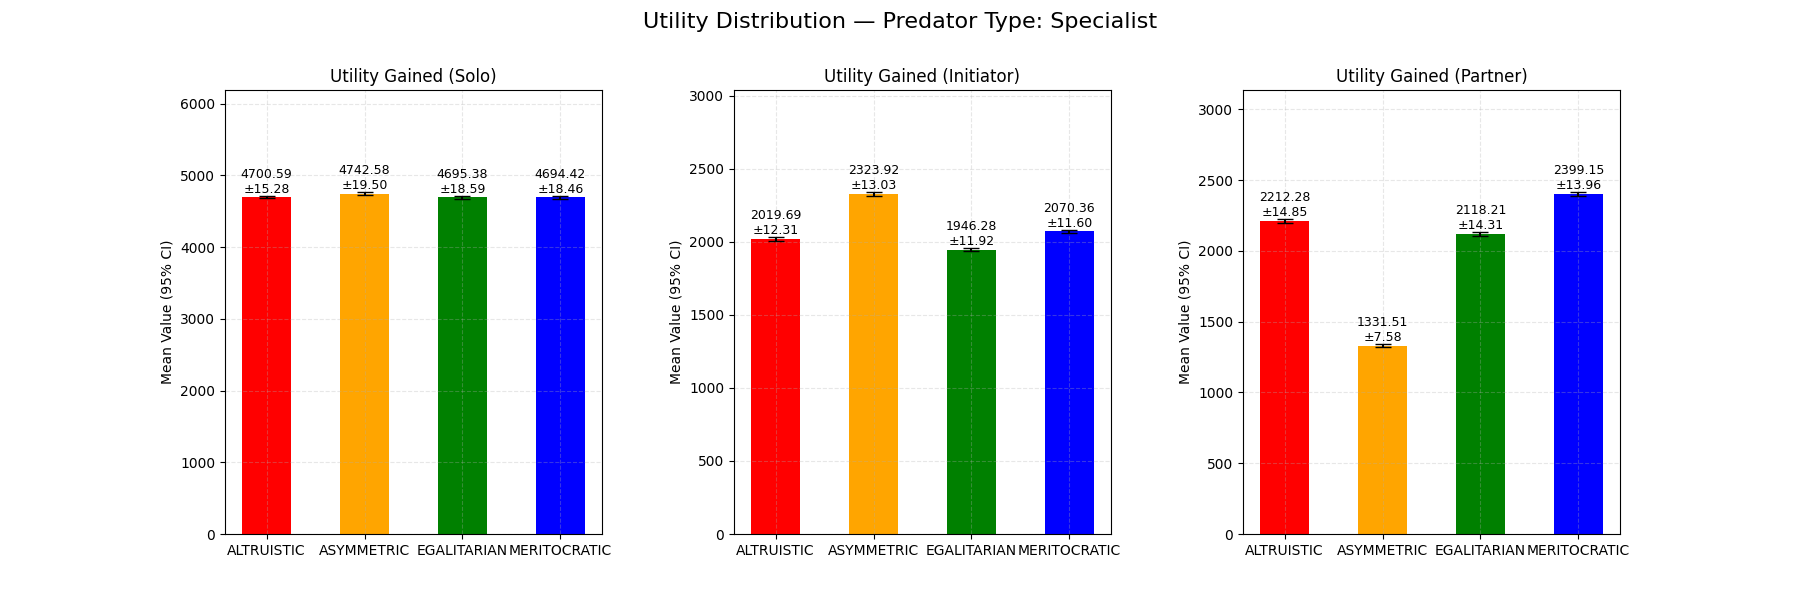
\includegraphics[width=1\textwidth]{EXP_3_SPECIALIST_10K_B.png}
		\caption{Specialist Predator - Utility Distribution (Heterogeneous, High Synergy).}
		\label{fig:exp_3_Specialist_B}
	\end{figure}
	
	\textbf{Freeloader Predators} \\
	
	Freeloader predators again show the clearest volume response to Asymmetric (66.64 coalition hunts), the highest for this type across any experiment but this time it is the fixed leader's share and not other high merit predators driving it. Since high synergy amplifies hunt success probabilities across the board, the flat leader's share split  becomes attractive precisely because it guarantees Freeloader a workable slice without depending on how its merit compares to a partner's. Finally, Freeloader's solo utility actually drops under Meritocratic, as high-synergy Meritocratic coalitions are so much more attractive than solo hunting that Freeloader shifts activity away from solo hunting entirely (116.34 solo hunts, its lowest), redirecting effort toward the tactic offering the largest capture probability gain even though its own merit-weighted share is low.
	
	\begin{figure}[H]
		\centering
		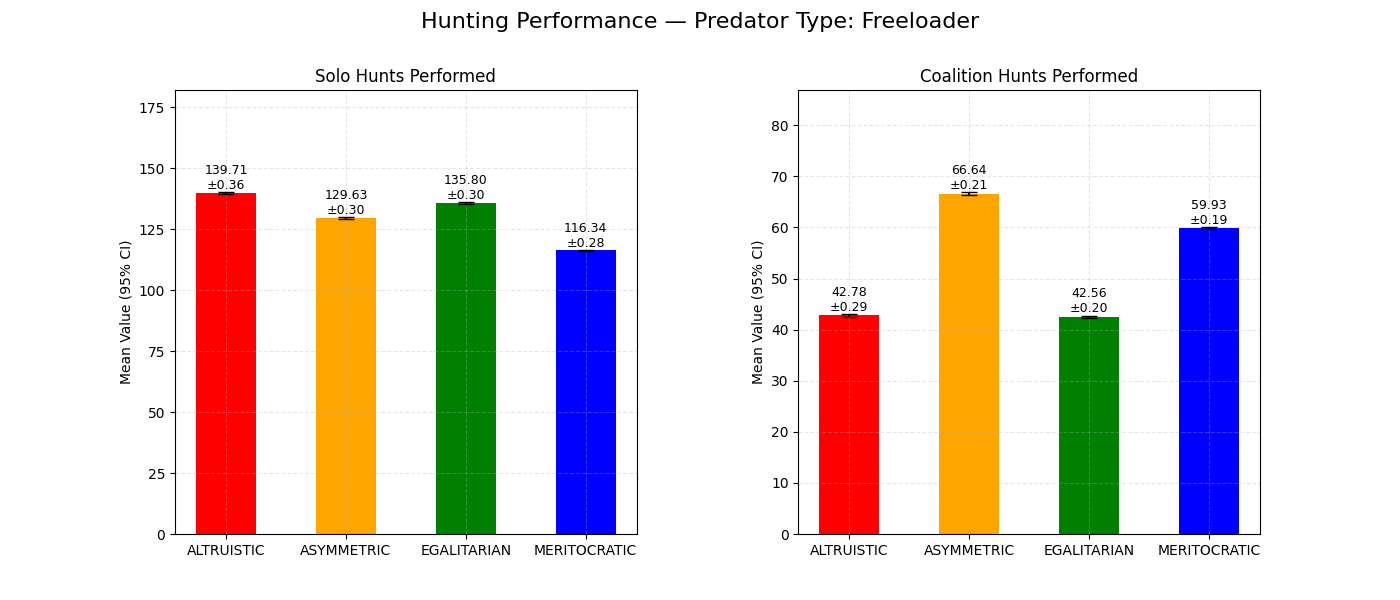
\includegraphics[width=1\textwidth]{EXP_3_FREELOADER_10K_A.png}
		\caption{Freeloader Predator - Hunting Performance (Heterogeneous, High Synergy).}
		\label{fig:exp_3_Freeloader_A}
	\end{figure}
	
	\begin{figure}[H]
		\centering
		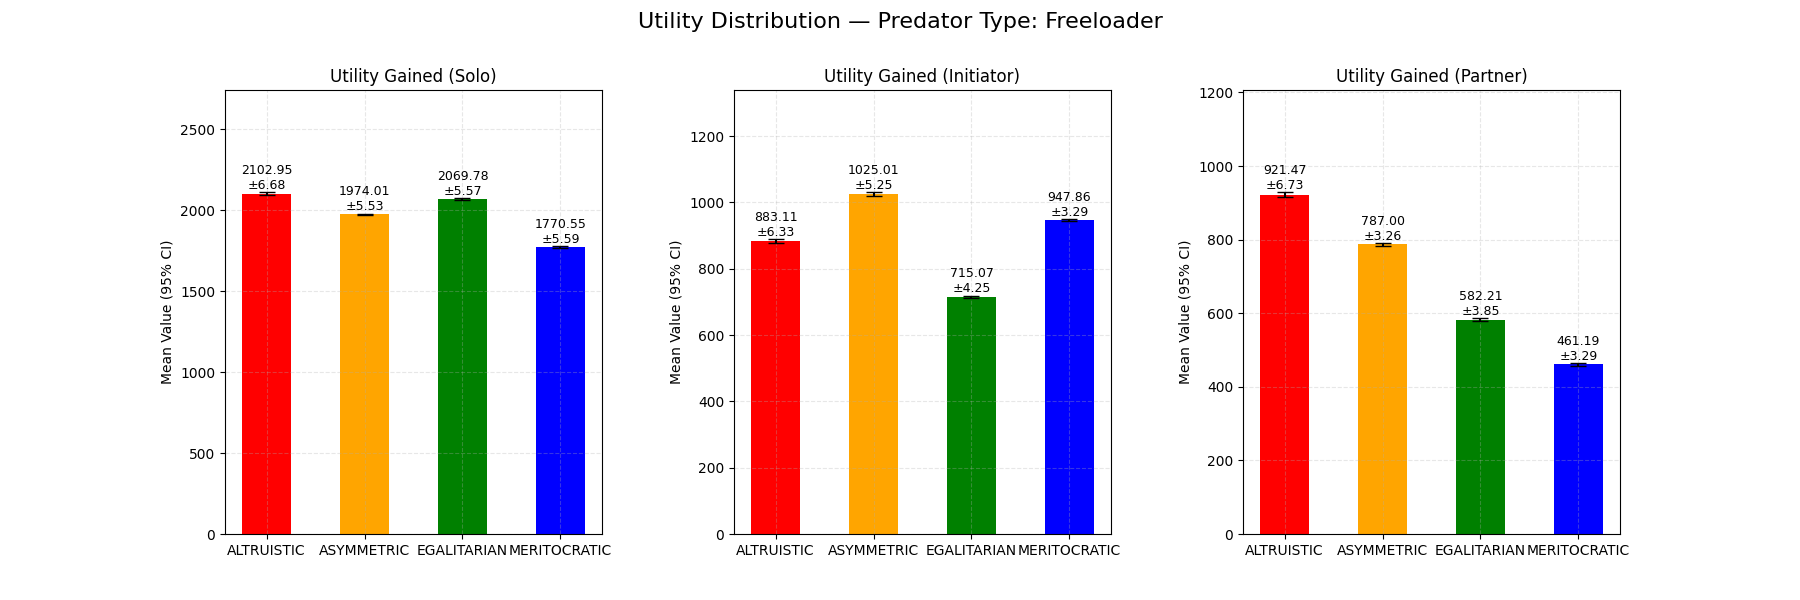
\includegraphics[width=1\textwidth]{EXP_3_FREELOADER_10K_B.png}
		\caption{Freeloader Predator - Utility Distribution (Heterogeneous, High Synergy).}
		\label{fig:exp_3_Freeloader_B}
	\end{figure}
	
	\textbf{Newbie Predators} \\
	
	Newbie predators show the strongest overall response to high synergy out of any type. Coalition hunt frequency almost doubles from the previous experiment. Since Newbie's bargaining threshold is constantly low, virtually every proposed share clears the bargaining check. However, high synergy also translates to high hunt success in cooperative hunts, so their utility check ( $E[U_{group}] \geq E[U_{solo}]$ ) is now satisfied far more easily too. The initiator/partner reversal seen in the previous experiment persists and intensifies, confirming that Newbie's structural role in this ecology is as a cheap, easily-satisfied recruit rather than a coalition organizer, a pattern that high synergy reinforces rather than corrects.
	
	\begin{figure}[H]
		\centering
		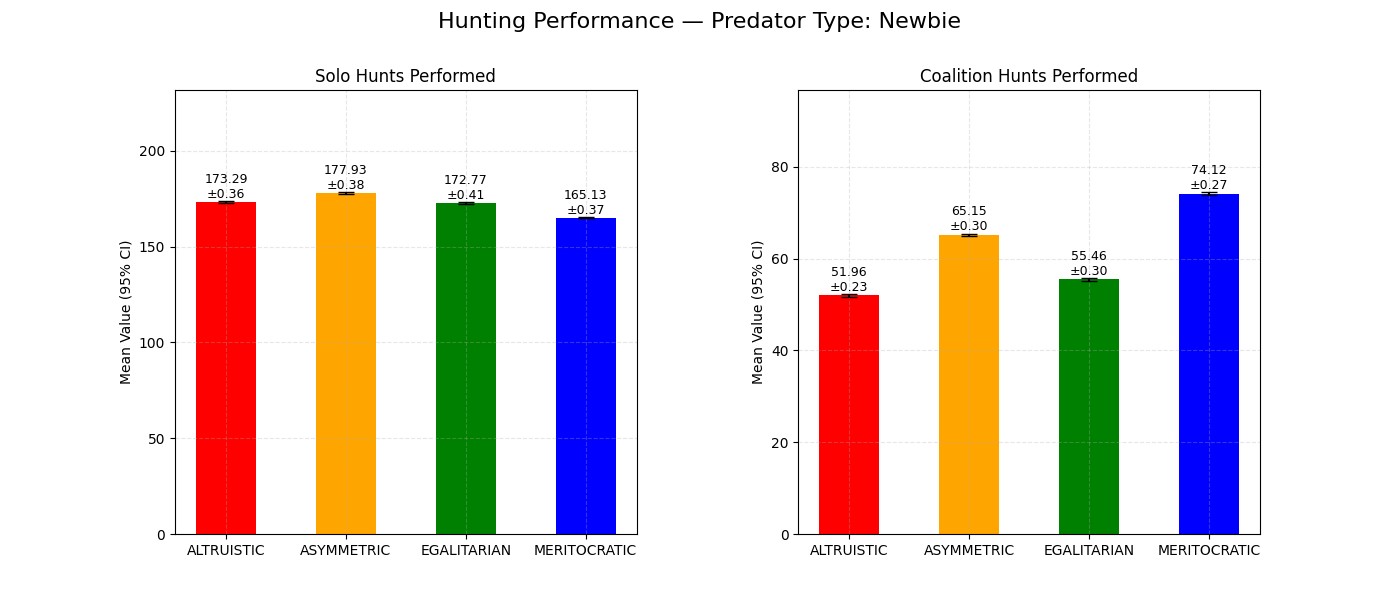
\includegraphics[width=1\textwidth]{EXP_3_NEWBIE_10K_A.png}
		\caption{Newbie Predator - Hunting Performance (Heterogeneous, High Synergy).}
		\label{fig:exp_3_Newbie_A}
	\end{figure}
	
	\begin{figure}[H]
		\centering
		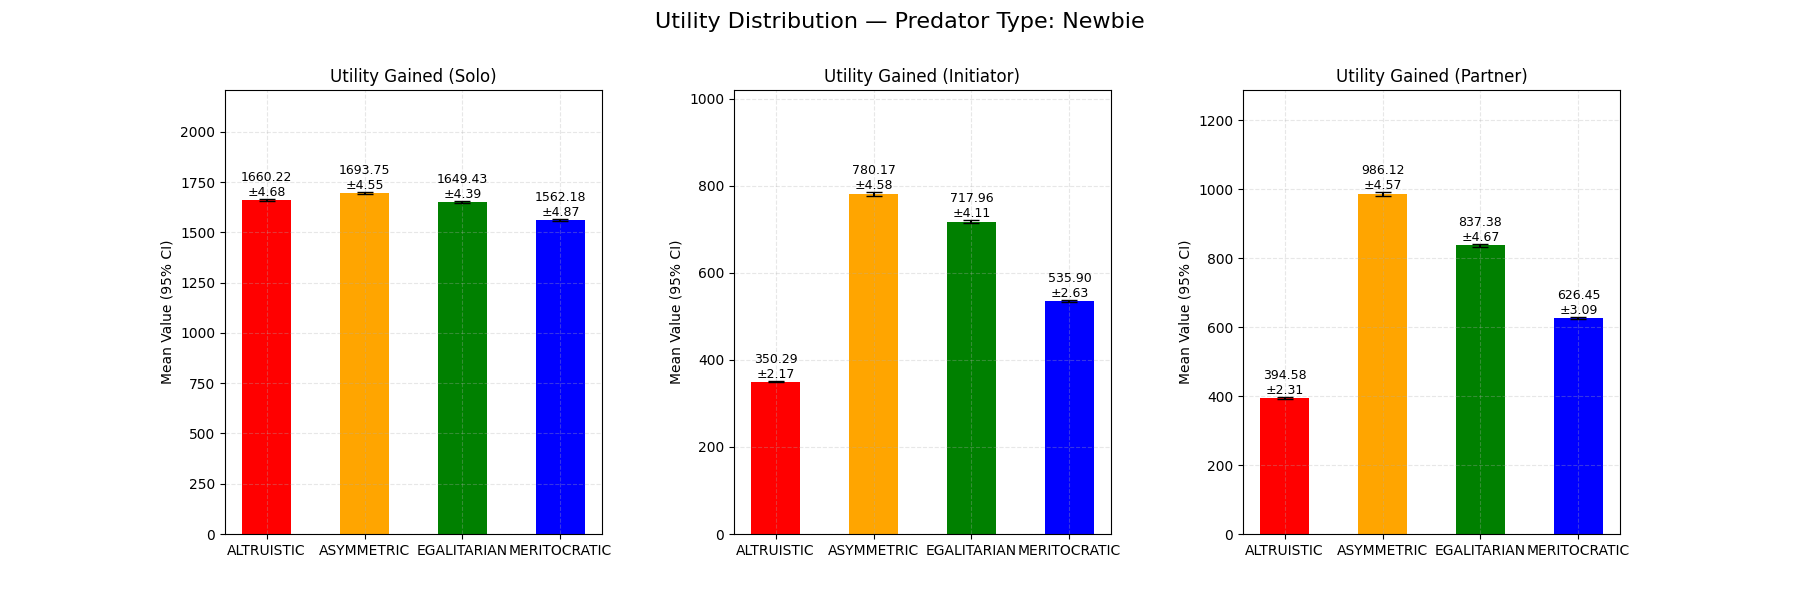
\includegraphics[width=1\textwidth]{EXP_3_NEWBIE_10K_B.png}
		\caption{Newbie Predator - Utility Distribution (Heterogeneous, High Synergy).}
		\label{fig:exp_3_Newbie_B}
	\end{figure}
	
	The Meritocratic tactic remains the top driver for cooperation on average (64.13) and wins outright for Baseline, Newbie, and Specialist. Asymmetric rises sharply to second place overall (58.37) and becomes the single best tactic for Freeloader. Egalitarian, notably, drops to last place on average as high synergy makes the flat split look worse to agents who could be extracting more via merit-weighting or by taking the leader's share in coalitions. Since coalition counts rise for everyone under every tactic once synergy doubles, utility gains rise as well across the board regardless of tactic. Synergy is a bigger factor than the tactic choice for raw output. But the equity gap widens specifically under Meritocratic. Specialist's utility advantage over the low-merit types grows even as their participation gap shrinks. This is the empirical core of the thesis's own claim that no amount of cooperative synergy can overcome the deterrent of a distribution tactic that rewards agents based on contribution alone. Synergy fixes who participates, not who benefits. Egalitarian is therefore the tactic that best protects social welfare in the equity sense under high synergy, even though it's no longer the top tactic for raw cooperation frequency.
	
	\begin{table}[H]
		\centering
		\begin{tabular}{|c|c|c|c|c|c|}
			\hline
			Tactic & Baseline & Specialist & Freeloader & Newbie & Total \\
			\hline
			Altruistic & 35.44 & 72.51 & 42.78 & 51.96 & 202.69 \\
			Asymmetric & 42.71 & 59.96 & \textbf{66.64} & 65.15 & 234.46 \\
			Egalitarian & 21.62 & 71.54 & 42.56 & 55.46 & 191.58 \\
			Meritocratic & \textbf{48.38} & \textbf{74.08} & 59.93 & \textbf{74.12} & \textbf{256.51} \\
			\hline
		\end{tabular}
		\caption{Average Coalition Frequency (Heterogeneous, High Synergy)}
	\end{table}
	
	\begin{table}[H]
		\centering
		\begin{tabular}{|c|c|c|c|c|c|}
			\hline
			Tactic & Baseline & Specialist & Freeloader & Newbie & Total \\
			\hline
			Altruistic & 678.30 & 2115.99 & 902.29 & 372.44 & 4069.02 \\
			Asymmetric & 797.62 & 1827.72 & \textbf{906.01} & \textbf{883.15} & 4414.50 \\
			Egalitarian & 539.71 & 2032.25 & 648.64 & 777.67 & 3998.27 \\
			Meritocratic & \textbf{981.90} & \textbf{2234.76} & 704.53 & 581.18 & \textbf{4502.37}\\
			\hline
		\end{tabular}
		\caption{Average Coalition Utility (Heterogeneous, High Synergy)}
	\end{table}
	
	\section {Experiments Conclusions}dgfdgdgdg
	
	In conclusion, Meritocratic is the single most reliable driver of coalition formation and cooperation across every condition tested. It wins for nearly every individual predator type in both heterogeneous experiments and is on par in the homogeneous experiment. This is the case because high merit predators result in more successful cooperative hunts on average that reward every participant, since it is rational enough for them even while their low merit is translated into a conservative share of the reward. Experiment 1 (homogeneous) shows this is not a property of the Meritocratic formula in isolation. Under equal parameters, Meritocratic, Egalitarian, and Altruistic are mathematically identical. It only emerges once real heterogeneity is introduced (Experiments 2 and 3). \\
	
	In terms of social welfare and utility gains, the three experiments together support a genuine trade-off rather than a single winner, and this is the thesis's central finding. If social welfare is determined by total utility extracted by the predator population, Meritocratic performs best, since it consistently maximizes coalition participation across all predator types and every successful coalition hunt is a raw increase of reward into the population that would otherwise not exist for low coalition frequency tactics. However, if social welfare is determined by fairness, broad-based benefit across the population, Egalitarian is the most robust choice. It is the only tactic whose formula is indifferent to merit or demand, so it never produces the divergence seen under Meritocratic, where high merit predators lead over low merit ones. Egalitarian never wins outright on raw output, but it never collapses for any type either. \\ 
	
	As it turns out, Altruistic functions as a targeted equity mechanism rather than a general-purpose welfare maximizer. It is specifically protective of the lowest merit types (Freeloader, Newbie) but never the best consistent performer, essentially subsidizing weak predators at the cost of the overall population throughput. Finally, Asymmetric is the most condition-dependent tactic: worst under homogeneity, mediocre under normal synergy, and surprisingly strong under high synergy for the Freeloader type since its fixed leader's share only becomes broadly acceptable once total coalition payoffs are large enough to absorb it. \\
	
%-----------------------------------------------------
%--------------- Serious Game Chapter ----------------
%-----------------------------------------------------
	\chapter{Serious Game Implementation}
	\label{ch:game}
	
	In this chapter we introduce the tactical elements of our proposed serious game. The setting is a virtual, growing community of cavemen, with the player being its chief and coordinator. \\
	\section{Hex Grid and Map Rendering}
	
	\section{Game Play}
	
	The core objective is the management of a communal food stockpile, which serves as the primary metric for the population's survival and growth. This stockpile decreases over time relative to the current population's upkeep, with a bigger food stockpile facilitating proportionally more population increase. \\
	
	The player is challenged to accommodate these needs through food collecting by creating and deploying autonomous "Predator" agents. Through the strategic deployment of these hunters, the game serves as an introduction to multi-agent AI environments, demonstrating how rational agents evaluate utility and engage in coalition formation. \\
	
	\subsection{Predator Management}
		
	Players create and send out predator hunters in the wilds. Following the environment;s principles from section 3, these Predators hunt rationally for their own benefit, either alone or in coalitions, using the same coalition formation framework. However, any excess food gained beyond their personal stockpile goes directly to the Player and the community. \\
	
	Every single characteristic is customizable by the Player alongside his negotiation tactic, since in this game setup they are not universal. These include: \\
	
	\begin{itemize}
		
		\item \textbf{Merit (Skill):} Defines the agent's productivity and contribution to a hunt.
		
		\item \textbf{Demand (Greed):} Defines the agent's basic demand for a reward share, directly influencing his effective demand factor in coalition negotiations.
		
		\item \textbf{Hunting Cost (Effort):} The food expenditure required for the predator to engage in a hunt.
		
		\item \textbf{Tactic (Negotiation):} The distribution tactic the predator uses to propose reward shares for a potential coalition. \\
		
	\end{itemize}
	
	Choosing the combination of parameters incurs a food cost and is bounded at a specific budget $K$ to avoid the creation of "super predators". Players may utilize predefined archetypes or develop customized load-outs. \\
	
	Inefficient predators can be recalled from the wilds with a minor penalty to their food stockpile. Depending on the distance $d$ from the recalled predator's hex to the Starting Hex, the refund to the player is its food stockpile, consuming what it needs to return to the starting hex: 
	
	\[ Refund(Recall) = F_{predator,i} - d * C_{move,i} \] \\
	
	To evaluate the performance of different predator configurations and negotiation tactics, the game system provides comprehensive data tracking. A dedicated statistics interface allows the player to monitor the success rates and food yields of various predator types. \\
	
	These visual aids, including graphs and performance metrics, enable the player to identify which combinations of Merit, Demand, Effort and Tactic that foster the most efficient coalitions. By analyzing these results, the player can observe how the "bargaining power" of agents—derived from their procedural rules and preferences—manifests in the game's economy. \\
	
	\subsection{Hex Exploration}
	
	To simulate stakes and spatial constraints, the game environment is also divided into a hexagonal grid. Predators begin in the Starting Hex and can only move into revealed hexes. Players must expend food to explore adjacent-to-explored Hexes, uncovering new areas and available prey. \\
	
	While prey populations are not hunted to total extinction, new prey have a chance to appear only upon Hex exploration. Thus, it is a functional requirement for predators to find new targets and maintain the community's growth. This spatial element adds a layer of strategy as clever clustering of explored areas may benefit the Player long term. \\
	
	\section{Guiding Tutorial}
	
	The educational component of this serious game is facilitated by "The Elder," an in-game guiding voice that provides strategic advice and technical orientation. The Elder interprets the complexities of agent behavior for the player, explaining why certain coalitions fail or succeed based on the hunters' characteristics. \\
	
	Through this interaction, the player learns the intricacies of coalition formation among rational agents. The tutorial emphasizes that success depends on creating incentives for cooperation, moving the community toward an "efficient equilibrium" or "full employment" state where synergy is maximized. \\
	
%-----------------------------------------------------
%---------------- Conclusion Chapter -----------------
%-----------------------------------------------------
	\chapter{Conclusion and Future Work}
	\label{ch:conclusion}
	In conclusion,
	
	Looking forward, there are several directions to follow for further research on this topic.
	
	\printbibliography
	
\end{document}